% !TeX spellcheck = en_GB
% !TeX encoding = UTF-8
% !TeX program = xelatex
% TODO Change language to en_GB (recommended) or en_US for English documents
\documentclass[11pt,a4paper,oneside]{report}             % Single-side
%\documentclass[11pt,a4paper,twoside,openright]{report}  % Duplex

% thanks to http://tex.stackexchange.com/a/47579/71109
\usepackage{ifxetex}
\usepackage{ifluatex}
\newif\ifxetexorluatex % a new conditional starts as false
\ifnum 0\ifxetex 1\fi\ifluatex 1\fi>0
   \xetexorluatextrue
\fi

\ifxetexorluatex
  \usepackage{fontspec}
\else
  \usepackage[T1]{fontenc}
  \usepackage[utf8]{inputenc}
  \usepackage[lighttt]{lmodern}
\fi

\usepackage[english,magyar]{babel} % Alapértelmezés szerint utoljára definiált nyelv lesz aktív, de később külön beállítjuk az aktív nyelvet.

%\usepackage{cmap}
\usepackage{amsfonts,amsmath,amssymb} % Mathematical symbols.
%\usepackage[ruled,boxed,resetcount,linesnumbered]{algorithm2e} % For pseudocodes. % beware: this is not compatible with LuaLaTeX, see http://tex.stackexchange.com/questions/34814/lualatex-and-algorithm2e
\usepackage{booktabs} % For publication quality tables for LaTeX
\usepackage{graphicx}

%\usepackage{fancyhdr}
%\usepackage{lastpage}

\usepackage{anysize}
%\usepackage{sectsty}
\usepackage{setspace} % For setting line spacing

\usepackage[unicode]{hyperref} % For hyperlinks in the generated document.
\usepackage{xcolor}
\usepackage{listings} % For source code snippets.

\usepackage[amsmath,thmmarks]{ntheorem} % Theorem-like environments.

\usepackage[hang]{caption}

\singlespacing

\newcommand{\selecthungarian}{
	\selectlanguage{magyar}
	\setlength{\parindent}{2em}
	\setlength{\parskip}{0em}
	\frenchspacing
}

\newcommand{\selectenglish}{
	\selectlanguage{english}
	\setlength{\parindent}{0em}
	\setlength{\parskip}{0.5em}
	\nonfrenchspacing
	\renewcommand{\figureautorefname}{Figure}
	\renewcommand{\tableautorefname}{Table}
	\renewcommand{\partautorefname}{Part}
	\renewcommand{\chapterautorefname}{Chapter}
	\renewcommand{\sectionautorefname}{Section}
	\renewcommand{\subsectionautorefname}{Section}
	\renewcommand{\subsubsectionautorefname}{Section}
}

\usepackage[numbers]{natbib}
\usepackage{xspace}


%TODO Set the main variables
\newcommand{\vikszerzoVezeteknev}{Wendl}
\newcommand{\vikszerzoKeresztnev}{Csongor}

\newcommand{\vikkonzulensAMegszolitas}{dr.~}
\newcommand{\vikkonzulensAVezeteknev}{Kovács}
\newcommand{\vikkonzulensAKeresztnev}{Tibor}

\newcommand{\vikkonzulensBMegszolitas}{}
\newcommand{\vikkonzulensBVezeteknev}{Konzulens}
\newcommand{\vikkonzulensBKeresztnev}{Kettő}

\newcommand{\vikkonzulensCMegszolitas}{}
\newcommand{\vikkonzulensCVezeteknev}{}
\newcommand{\vikkonzulensCKeresztnev}{}

\newcommand{\vikcim}{Urban traffic simulation using modern technologies} % Cím
\newcommand{\viktanszek}{\bmeaut} % Tanszék
\newcommand{\vikdoktipus}{\bsc} % Dokumentum típusa (\bsc vagy \msc)
\newcommand{\vikmunkatipusat}{szakdolgozatot} % a "hallgató nyilatkozat" részhez: szakdolgozatot vagy diplomatervet

\newcommand{\szerzoMeta}{\vikszerzoVezeteknev{} \vikszerzoKeresztnev} % egy szerző esetén
%\newcommand{\szerzoMeta}{\vikszerzoVezeteknev{} \vikszerzoKeresztnev, \tdkszerzoB} % két szerző esetén

%TODO Language configuration -- choose one
% Beállítások magyar nyelvű dolgozathoz
%%--------------------------------------------------------------------------------------
% Elnevezések
%--------------------------------------------------------------------------------------
\newcommand{\bme}{Budapesti Műszaki és Gazdaságtudományi Egyetem}
\newcommand{\vik}{Villamosmérnöki és Informatikai Kar}

\newcommand{\bmeaut}{Automatizálási és Alkalmazott Informatikai Tanszék}

\newcommand{\keszitette}{Készítette}
\newcommand{\konzulens}{Konzulens}

\newcommand{\bsc}{Szakdolgozat}
\newcommand{\msc}{Diplomaterv}
\newcommand{\tdk}{TDK dolgozat}
\newcommand{\bsconlab}{BSc Önálló laboratórium}
\newcommand{\msconlabi}{MSc Önálló laboratórium 1.}
\newcommand{\msconlabii}{MSc Önálló laboratórium 2.}

\newcommand{\pelda}{Példa}
\newcommand{\definicio}{Definíció}
\newcommand{\tetel}{Tétel}

\newcommand{\bevezetes}{Bevezetés}
\newcommand{\koszonetnyilvanitas}{Köszönetnyilvánítás}
\newcommand{\fuggelek}{Függelék}

% Opcionálisan átnevezhető címek
%\addto\captionsmagyar{%
%\renewcommand{\listfigurename}{Saját ábrajegyzék cím}
%\renewcommand{\listtablename}{Saját táblázatjegyzék cím}
%\renewcommand{\bibname}{Saját irodalomjegyzék név}
%}

\newcommand{\szerzo}{\vikszerzoVezeteknev{} \vikszerzoKeresztnev}
\newcommand{\vikkonzulensA}{\vikkonzulensAMegszolitas\vikkonzulensAVezeteknev{} \vikkonzulensAKeresztnev}

\newcommand{\selectthesislanguage}{\selecthungarian}

\bibliographystyle{huplain}

\def\lstlistingname{lista}

\newcommand{\appendixnumber}{6}  % a fofejezet-szamlalo az angol ABC 6. betuje (F) lesz

% Settings for English documents
%--------------------------------------------------------------------------------------
% Elnevezések
%--------------------------------------------------------------------------------------
\newcommand{\bme}{Budapest University of Technology and Economics}
\newcommand{\vik}{Faculty of Electrical Engineering and Informatics}

\newcommand{\bmemit}{Department of Measurement and Information Systems}

\newcommand{\keszitette}{Author}
\newcommand{\konzulens}{Advisor}

\newcommand{\bsc}{Bachelor's Thesis}
\newcommand{\msc}{Master's Thesis}
\newcommand{\tdk}{Scientific Students' Association Report}
\newcommand{\bsconlab}{BSc Project Laboratory}
\newcommand{\msconlabi}{MSc Project Laboratory 1}
\newcommand{\msconlabii}{MSc Project Laboratory 2}

\newcommand{\pelda}{Example}
\newcommand{\definicio}{Definition}
\newcommand{\tetel}{Theorem}

\newcommand{\bevezetes}{Introduction}
\newcommand{\koszonetnyilvanitas}{Acknowledgements}
\newcommand{\fuggelek}{Appendix}

% Optional custom titles
%\addto\captionsenglish{%
%\renewcommand*{\listfigurename}{Your list of figures title}
%\renewcommand*{\listtablename}{Your list of tables title}
%\renewcommand*{\bibname}{Your bibliography title}
%}

\newcommand{\szerzo}{\vikszerzoKeresztnev{} \vikszerzoVezeteknev}
\newcommand{\vikkonzulensA}{\vikkonzulensAMegszolitas\vikkonzulensAKeresztnev{} \vikkonzulensAVezeteknev}
\newcommand{\vikkonzulensB}{\vikkonzulensBMegszolitas\vikkonzulensBKeresztnev{} \vikkonzulensBVezeteknev}
\newcommand{\vikkonzulensC}{\vikkonzulensCMegszolitas\vikkonzulensCKeresztnev{} \vikkonzulensCVezeteknev}

\newcommand{\selectthesislanguage}{\selectenglish}

\bibliographystyle{plainnat}

\newcommand{\ie}{i.e.\@\xspace}
\newcommand{\Ie}{I.e.\@\xspace}
\newcommand{\eg}{e.g.\@\xspace}
\newcommand{\Eg}{E.g.\@\xspace}
\newcommand{\etal}{et al.\@\xspace}
\newcommand{\etc}{etc.\@\xspace}
\newcommand{\vs}{vs.\@\xspace}
\newcommand{\viz}{viz.\@\xspace} % videlicet
\newcommand{\cf}{cf.\@\xspace} % confer
\newcommand{\Cf}{Cf.\@\xspace}
\newcommand{\wrt}{w.r.t.\@\xspace} % with respect to
\newcommand{\approximately}{approx.\@\xspace}

\newcommand{\appendixnumber}{1}  % a fofejezet-szamlalo az angol ABC 1. betuje (A) lesz

%--------------------------------------------------------------------------------------
% Page layout setup
%--------------------------------------------------------------------------------------
% we need to redefine the pagestyle plain
% another possibility is to use the body of this command without \fancypagestyle
% and use \pagestyle{fancy} but in that case the special pages
% (like the ToC, the References, and the Chapter pages)remain in plane style

\pagestyle{plain}
\marginsize{35mm}{25mm}{15mm}{15mm}

\setcounter{tocdepth}{3}
%\sectionfont{\large\upshape\bfseries}
\setcounter{secnumdepth}{3}

\sloppy % Margón túllógó sorok tiltása.
\widowpenalty=10000 \clubpenalty=10000 %A fattyú- és árvasorok elkerülése
\def\hyph{-\penalty0\hskip0pt\relax} % Kötőjeles szavak elválasztásának engedélyezése


%--------------------------------------------------------------------------------------
% Setup hyperref package
%--------------------------------------------------------------------------------------
\hypersetup{
    % bookmarks=true,            % show bookmarks bar?
    unicode=true,              % non-Latin characters in Acrobat's bookmarks
    pdftitle={\vikcim},        % title
    pdfauthor={\szerzoMeta},    % author
    pdfsubject={\vikdoktipus}, % subject of the document
    pdfcreator={\szerzoMeta},   % creator of the document
    pdfproducer={},    % producer of the document
    pdfkeywords={},    % list of keywords (separate then by comma)
    pdfnewwindow=true,         % links in new window
    colorlinks=true,           % false: boxed links; true: colored links
    linkcolor=black,           % color of internal links
    citecolor=black,           % color of links to bibliography
    filecolor=black,           % color of file links
    urlcolor=black             % color of external links
}

\usepackage{graphicx,wrapfig,dirtytalk}
\usepackage{pgfplots}
\usepackage{amsmath}

\pgfplotsset{compat=1.18}
%--------------------------------------------------------------------------------------
% Set up listings
%--------------------------------------------------------------------------------------
\definecolor{lightgray}{rgb}{0.95,0.95,0.95}
\lstset{
	basicstyle=\scriptsize\ttfamily, % print whole listing small
	keywordstyle=\color{black}\bfseries, % bold black keywords
	identifierstyle=, % nothing happens
	% default behavior: comments in italic, to change use
	% commentstyle=\color{green}, % for e.g. green comments
	stringstyle=\scriptsize,
	showstringspaces=false, % no special string spaces
	aboveskip=3pt,
	belowskip=3pt,
	backgroundcolor=\color{lightgray},
	columns=flexible,
	keepspaces=true,
	escapeinside={(*@}{@*)},
	captionpos=b,
	breaklines=true,
	frame=single,
	float=!ht,
	tabsize=2,
	literate=*
		{á}{{\'a}}1	{é}{{\'e}}1	{í}{{\'i}}1	{ó}{{\'o}}1	{ö}{{\"o}}1	{ő}{{\H{o}}}1	{ú}{{\'u}}1	{ü}{{\"u}}1	{ű}{{\H{u}}}1
		{Á}{{\'A}}1	{É}{{\'E}}1	{Í}{{\'I}}1	{Ó}{{\'O}}1	{Ö}{{\"O}}1	{Ő}{{\H{O}}}1	{Ú}{{\'U}}1	{Ü}{{\"U}}1	{Ű}{{\H{U}}}1
}


%--------------------------------------------------------------------------------------
% Set up theorem-like environments
%--------------------------------------------------------------------------------------
% Using ntheorem package -- see http://www.math.washington.edu/tex-archive/macros/latex/contrib/ntheorem/ntheorem.pdf

\theoremstyle{plain}
\theoremseparator{.}
\newtheorem{example}{\pelda}

\theoremseparator{.}
%\theoremprework{\bigskip\hrule\medskip}
%\theorempostwork{\hrule\bigskip}
\theorembodyfont{\upshape}
\theoremsymbol{{\large \ensuremath{\centerdot}}}
\newtheorem{definition}{\definicio}

\theoremseparator{.}
%\theoremprework{\bigskip\hrule\medskip}
%\theorempostwork{\hrule\bigskip}
\newtheorem{theorem}{\tetel}


%--------------------------------------------------------------------------------------
% Some new commands and declarations
%--------------------------------------------------------------------------------------
\newcommand{\code}[1]{{\upshape\ttfamily\scriptsize\indent #1}}
\newcommand{\doi}[1]{DOI: \href{http://dx.doi.org/\detokenize{#1}}{\raggedright{\texttt{\detokenize{#1}}}}} % A hivatkozások közt így könnyebb DOI-t megadni.

\DeclareMathOperator*{\argmax}{arg\,max}
%\DeclareMathOperator*[1]{\floor}{arg\,max}
\DeclareMathOperator{\sign}{sgn}
\DeclareMathOperator{\rot}{rot}


%--------------------------------------------------------------------------------------
% Setup captions
%--------------------------------------------------------------------------------------
\captionsetup[figure]{
	width=.85\textwidth,
	aboveskip=10pt}

\renewcommand{\captionlabelfont}{\bf}
%\renewcommand{\captionfont}{\footnotesize\it}

%--------------------------------------------------------------------------------------
% Hyphenation exceptions
%--------------------------------------------------------------------------------------
\hyphenation{Shakes-peare Mar-seilles ár-víz-tű-rő tü-kör-fú-ró-gép}


\author{\vikszerzo}
\title{\viktitle}

%--------------------------------------------------------------------------------------
% Table of contents and the main text
%--------------------------------------------------------------------------------------
\begin{document}

\pagenumbering{gobble}

\selectthesislanguage

\hypersetup{pageanchor=false}
%--------------------------------------------------------------------------------------
%	The title page
%--------------------------------------------------------------------------------------
\begin{titlepage}
\begin{center}

\includegraphics[width=60mm,keepaspectratio]{figures/bme_logo.pdf}\\
\vspace{0.3cm}
\textbf{\bme}\\
\textmd{\vik}\\
\textmd{\viktanszek}\\[5cm]

\vspace{0.4cm}
{\huge \bfseries \vikcim}\\[0.8cm]
\vspace{0.5cm}
\textsc{\Large \vikdoktipus}\\[4cm]

{
	\renewcommand{\arraystretch}{0.85}
	\begin{tabular}{cc}
	 \makebox[7cm]{\emph{\keszitette}} & \makebox[7cm]{\emph{\konzulens}} \\ \noalign{\smallskip}
	 \makebox[7cm]{\szerzo} & \makebox[7cm]{\vikkonzulensA} \\
	\end{tabular}
}

\vfill
{\large \today}
\end{center}
\end{titlepage}
\hypersetup{pageanchor=false}

		   % Szakdolgozat/Diplomaterv címlap


% Table of Contents
%~~~~~~~~~~~~~~~~~~~~~~~~~~~~~~~~~~~~~~~~~~~~~~~~~~~~~~~~~~~~~~~~~~~~~~~~~~~~~~~~~~~~~~
\tableofcontents\vfill


% Declaration and Abstract
%~~~~~~~~~~~~~~~~~~~~~~~~~~~~~~~~~~~~~~~~~~~~~~~~~~~~~~~~~~~~~~~~~~~~~~~~~~~~~~~~~~~~~~
\selectlanguage{magyar}
\pagenumbering{gobble}
%--------------------------------------------------------------------------------------
% Nyilatkozat
%--------------------------------------------------------------------------------------
\begin{center}
\large
\textbf{HALLGATÓI NYILATKOZAT}\\
\end{center}

Alulírott \emph{\vikszerzoVezeteknev{} \vikszerzoKeresztnev}, szigorló hallgató kijelentem, hogy ezt a \vikmunkatipusat{} meg nem engedett segítség nélkül, saját magam készítettem, csak a megadott forrásokat (szakirodalom, eszközök stb.) használtam fel. Minden olyan részt, melyet szó szerint, vagy azonos értelemben, de átfogalmazva más forrásból átvettem, egyértelműen, a forrás megadásával megjelöltem.

Hozzájárulok, hogy a jelen munkám alapadatait (szerző(k), cím, angol és magyar nyelvű tartalmi kivonat, készítés éve, konzulens(ek) neve) a BME VIK nyilvánosan hozzáférhető elektronikus formában, a munka teljes szövegét pedig az egyetem belső hálózatán keresztül (vagy autentikált felhasználók számára) közzétegye. Kijelentem, hogy a benyújtott munka és annak elektronikus verziója megegyezik. Dékáni engedéllyel titkosított diplomatervek esetén a dolgozat szövege csak 3 év eltelte után válik hozzáférhetővé.

\begin{flushleft}
\vspace*{1cm}
Budapest, \today
\end{flushleft}

\begin{flushright}
 \vspace*{1cm}
 \makebox[7cm]{\rule{6cm}{.4pt}}\\
 \makebox[7cm]{\emph{\vikszerzoVezeteknev{} \vikszerzoKeresztnev}}\\
 \makebox[7cm]{hallgató}
\end{flushright}
\thispagestyle{empty}

\vfill
\clearpage
\thispagestyle{empty} % an empty page

\selectthesislanguage
 %TODO Hallgatói nyilatkozat -- TDK és OTDK esetén törlendő!
\pagenumbering{roman}
\setcounter{page}{1}

\selecthungarian

%----------------------------------------------------------------------------
% Abstract in Hungarian
%----------------------------------------------------------------------------
\chapter*{Kivonat}\addcontentsline{toc}{chapter}{Kivonat}

Jelen dokumentum egy diplomaterv sablon, amely formai keretet ad a BME Villamosmérnöki és Informatikai Karán végző hallgatók által elkészítendő szakdolgozatnak és diplomatervnek. A sablon használata opcionális. Ez a sablon \LaTeX~alapú, a \emph{TeXLive} \TeX-implementációval és a PDF-\LaTeX~fordítóval működőképes.


\vfill
\selectenglish


%----------------------------------------------------------------------------
% Abstract in English
%----------------------------------------------------------------------------
\chapter*{Abstract}\addcontentsline{toc}{chapter}{Abstract}

This document is a \LaTeX-based skeleton for BSc/MSc~theses of students at the Electrical Engineering and Informatics Faculty, Budapest University of Technology and Economics. The usage of this skeleton is optional. It has been tested with the \emph{TeXLive} \TeX~implementation, and it requires the PDF-\LaTeX~compiler.


\vfill
\selectthesislanguage

\newcounter{romanPage}
\setcounter{romanPage}{\value{page}}
\stepcounter{romanPage}    %TODO Összefoglaló -- TDK és OTDK esetén nem kötelező


% The main part of the thesis
%~~~~~~~~~~~~~~~~~~~~~~~~~~~~~~~~~~~~~~~~~~~~~~~~~~~~~~~~~~~~~~~~~~~~~~~~~~~~~~~~~~~~~~
\pagenumbering{arabic}

\chapter{Preface}

\section{Motivation}

The world these days is more urbanised than ever, and the trend of people moving to cities is expected to continue in the following decades. With individual car travel proving ever more wasteful -- both financially and environmentally -- as population density increases, policymakers and urban planners need to make public transport and bicycling more convenient for the average citizen. The needs of cities are ever-changing, and without sufficient data, this is an impossible task. Planners should have access to adequate tools to aid decision making.

Personally, I've seen multiple enterprise programs in related fields that left me quite disappointed. User interfaces are typically clunky and remnants of early 2000s software. Automating even small tasks can be very difficult, and each action takes a long time to execute. In a way, they remind me of the old versions of word processors and spreadsheet editors.

I wanted to try my hand at creating something in the transit analysis field that would improve on these issues. I didn't want to start with the expectation of replacing a popular software solution, so I intended to make something that would have entertainment value, while providing a platform for professional applications.


\section{Goals and requirements}

The aim of this project is to provide a three-dimensional map using open source data, and to create a visualisation tool on top of that. The city's buildings should be distinguishable, both with their shapes as well as available metadata, such as addresses or year of construction. The user should be able to move around the viewpoint, zoom in or out, and select buildings to inspect them. The software should be able to run a simulation of inhabitants and show the most popular areas in the city. It must be possible to load different cities from files encoded using a standard protocol, but only one city needs to be active at a time.

The app shall be divided into layers that resemble a usual server-client architecture. Communication should be done using standard public protocols, but data does not need to be published to arbitrary HTTP clients. The client should not hold more information than is required for the visualisation; computation-heavy tasks need to be offloaded to the server. The graphical capabilities of the app shall not have hardware-specific requirements, such as Nvidia's RTX. The layers should be able to run on the same computer, or entirely different machines too. The program should be able to run on the Windows, Linux and Mac desktop operating systems. A single server should respond to multiple clients at once.

The user interface must be understandable by people without a technical background, it should give feedback for actions taken. The technologies used should be maintainable and up to date. The software should also be distributable in a containerised form, for a zero-friction installation.

Performance should be a priority and a city with two million real life inhabitants should be loadable and navigable on a consumer-grade computer. The number of supported agents should be enough to show statistical significance.
\chapter{The current state of the transit modelling industry}
The purpose of modelling public transit systems is two-fold: evaluating current service patterns and discovering new routes are equally as important. The overall task is usually treated as a datamining exercise. As such, data collection is paramount, with presentation being of secondary concern. Just like in politics, a smaller but well-rounded dataset can allow us to make predictions and conclusions about the whole of a system.

Throughout this section, I'll introduce state of the art data collection and modelling solutions. Wherever appropriate, I will also show examples pertaining to my home city, Budapest.

\section{Data collection}
\subsection{Traditional, in-person method}

Up until the mid-2010s, the main method of collecting information was passenger counting. Employees could often be seen at bus stops or train stations with a clipboard, tracking the flow of commuters throughout the day, often at multiple stops along a single line. This allowed the recorded numbers to be imported into spreadsheet software, resulting in charts that show passenger density or even their distribution according to certain parameters.

Despite its limited scope, this approach has a few advantages. Data is rarely faulty as there is nothing in the loop that could technically malfunction. By hand-picking the numbers to record, it's possible to analyse an interchange in-depth; for example, to find out the amount of people boarding trains after leaving a specific underpass exit. More specific data can also be recorded about transit users, such as their age, gender and carried luggage.

The downsides however, are easy to see. The ongoing costs may be high due to employee compensation. It's also nearly impossible to cover a sufficiently large percentage of the system, lots of extrapolation is needed, which affects accuracy. In 2024, in-person counting has taken on an auxiliary role, only used as an additional measure or in technically challenging situations.

\subsection{Physical counting}

In 1983, the Budapest Transport Privately Held Corporation (BKV Zrt.) purchased simple computers from the Austrian Knorr-Bremse company, capable of measuring and interpreting the pressure placed on a bus' hydraulic system.\cite{ik260_article} With known baseline values, the current passenger count could be guessed with decent precision when travelling between any two stops. The numbers could then be used when planning new timetable assignments -- to increase or decrease headway between subsequent vehicles. The computers have mostly gone, as a result of local modernisation efforts.

Road vehicles, including cars and bicycles can be tallied using traffic induction loops.\cite{fhwaLoop} In use since the 1960s, these are simple circuits including an insulated wire placed into the road surface by sawing or otherwise cutting the asphalt. Whenever a vehicle drives over the wire, the inductivity changes. By attaching a simple processor, the frequency and length of signals can be mapped to different vehicle classes -- a semi truck and family sedan have entirely different signatures.

Budapest has around seven hundred induction loops that give a comprehensive, near-realtime picture of the city's traffic. Around fifty cameras provide a visual aid.\cite{BkkDataCollection}

\subsection{Digital counting}
Camera picture analysis reveals a lot about an junction's dominant flow direction. Accurate numbers exist on a per-lane basis. This field is exciting in its own right, as data sanitisation, object detection and machine inference is highly applicable here.

Many cities around the world currently use automated passenger counting to inform decisions. Examples include London (TfL), Berlin (BVG) and Chicage (CTA). The usual solution includes infrared sensors mounted above the doors of certain vehicles. These detectors can count boarding and disembarking people in real time, and upload this information to a central database.

Aside from the already mentioned purpose of timetable planning, this data can be used to handle overcrowding events -- such as a football match or live show -- by deploying more vehicles to increase capacity. As the devices are hooked into the vehicle's onboard computer, the numbers can be correlated with the location and time. CCTV cameras often act as a secondary source or means of verification for these schemes.

With the rise of online and mobile journey planner applications, users themselves can be the source of statistics. Multiple passengers searching for the same destination, or the use of ticketing and geolocation functions within an app can be treated as patterns to investigate. Built-in reporting systems, such as Google's analytics (available on Firebase) help spread this practice.

\section{City modelling}

Processing usage numbers is usually a fairly conventional affair (using spreadsheets, graphing the data, or utilising some form of machine learning), but designing roads, transport lines and vehicles that fulfil the needs of a city usually requires specialist software. I'll introduce the professional tool and the video game that inspired my work.

Cities Skylines is a single-player city-builder game developed by Colossal Order and published by Paradox Interactive in 2015. The game is a spiritual successor to the SimCity franchise, discontinued in 2013. The player's task is to build a town and metropolitan area from the ground up, requiring a decent sense of economics. The game is known for its detailed and at times challenging to render graphics on any zoom level. Cities are divided into residential, commercial, industrial and office zones, denoted with the now traditional colour scheme of green-blue-yellow.

While not intended for professional use, the simulation system, coupled with countless available community mods make it a strong contender for quick iterations on real life cities. Each member of the population constantly makes decisions on travelling and their living situation, moving homes when it's advisable. Traffic management is very important, as commercial buildings require lots of freight trucks in order to get goods. This mirrors real-life zoning concepts and forces a hierarchical road system to be built. Since I've played the game for over 100 hours, it's what influenced the project the most. I made use of the zoning colours and incorporated individual building information pages, as well as a version of the game's camera system. Initially, it was a full recreation of the smoothened three-dimensional camera, but I ended up going for a top-down view, as this looked much better with the final heatmap.

PTV Visum is a more involved, planning-focused software used by transit agencies, such as the Swiss Federal Railways. The app merges real socio-economic data and highly detailed transit models to predict trends. Cost analysis and fleet planning is also supported. It's well known for a very high level of detail, but this means sacrifices in performance and the user interface, which mostly reminds me of the 2012 version of Microsoft's Visual Studio. The maps are nevertheless highly detailed, with nodes and links that act similarly to OpenStreetMap's data. Visum places a strong emphasis on traffic simulation, with custom scenarios that can be compared to real trends easily. Multimodal (such as park and ride) travel is also supported. The main idea I used was the non-realtime evaluation of assignments; my heatmaps are calculated similarly, with only the result being shown. %CONSIDERED DONE
%----------------------------------------------------------------------------
\chapter{Felhasznált eszközök}
\label{sec:LatexTools}

Munkámat a JVM-ökoszisztéma eszközeivel végeztem, szem előtt tartva a kiírásban kulcsfontosságú elemként rögzített modernitást, a kompatibilitást és a hordozhatóságot. Ennek megfelelően ahol lehetséges, kerültem a jövőbeli eltávolításra kijelölt programelemek használatát, illetve az instabil verzióktól függést.
%----------------------------------------------------------------------------
\section{Kotlin \raisebox{-1ex}{
\includegraphics[width=8mm, keepaspectratio]{images/kotlin_logo.png}}}

%----------------------------------------------------------------------------
A Kotlin multiplatform, statikusan típusos, több paradigmát támogató programozási nyelv. Specifikációját a JetBrains rendszeresen frissített, publikus, bárki által megtekinthető formában teszi közzé.~\cite{KotlinSpec} Az első prototípus verzió 2011-ben került kiadásra, és mindössze egy évvel később nyílt forráskódú projektté alakult. Az első éles kiadását 2016-ban érte el a nyelv, 2017-től hivatalosan támogatott az Android mobil operációs rendszerre írt alkalmazások terén, 2019 óta pedig az Android elsődleges nyelve.~\cite{KotlinPast}

Népszerűségét elsősorban az intuitív szintaxisának és a JVM-mel\footnote{JVM: \@Java Virtual Machine, jelenleg az Oracle tulajdonában lévő, szabvánnyal specifikált futtatómotor, elsősorban a Java nyelven írt programok futtatásához } való már-már tökéletes kompatibilitásának köszönheti. Bármilyen Java-ban írt kódrészlet felhasználható külső referenciaként egy Kotlin programban, a programozó közösség által készített számtalan Java könyvtár így kiaknázható marad.  Egy projekten belül nincs korlátozás a két nyelv forrásfájljainak megoszlására; érdemes viszont megjegyezni, hogy a kompatibilitás egyirányú. Java kódból nem lehet visszahívni Kotlin kódba.

A megírt programok fordítási és optimalizálási fázisokon mennek keresztül, mielőtt futtatható állományok vagy eszköztárak készülnek belőlük. A Kotlin fordítómotorjával készített binárisok közel azonos teljesítményűek hagyományos JVM megfelelőikhez képest. A JVM-en kívül más fordítási célok is léteznek:
\begin{itemize}
    \item Kotlin/Native (2023 óta stabil, számos operációs rendszerre biztosít natív, futtató virtuális gépet nem igénylő megoldást)
    \item Kotlin/JS (a megírt kódot JavaScript-re fordítjuk, így egy fordítást igénylő nyelvből interpretált kódot készíthetünk; webböngészőhöz ideális)
\end{itemize}

A nyelv alapvetően egyszerű kódstruktúrájú, jól értelmezhető és gyorsan írható. Emellett a frusztráló, sok esetben hátráltató szintaktikai és programtechnikai elemek közül sokat elhagytak a fejlesztők -- erre és a funkcionális paradigma által nyújtott lehetőségekre a későbbiekben számos példát fogok mutatni kódrészleteken keresztül.

Szakdolgozatom elkészítéséhez a legfrissebb, 2.0.21-es verziót használtam a JetBrains saját, IntelliJ Idea néven futó programján keresztül. A felhasznált JVM változat a legújabb stabilnak tekinthető 23-as főverzió Oracle OpenJDK implementációja; a program által garantált abszolút minimális verzió a 2023 szeptemberében kiadott 21-es LTS\footnote{Long Term Support, a szoftverfejlesztés körében a kiadó által az adott verzióval kapcsolatban vállalt hosszabb idejű, több éves támogatást jelent} változat, ennek a főágú támogatása 2028-ban ér véget.~\cite{JavaRoadmap} %DONE
\chapter{Data sources} %TODO rename

\section{OpenStreetMap}

OpenStreetMap (OSM) is a collaborative community project to create a full, editable representation of our world. The project was founded in 2004 by Steve Coast, and now boasts over ten million registered volunteer users providing data from around the globe. Unlike proprietary services (such as Google Maps or Apple Maps), OSM data is open and freely available to build on or modify.\cite{osmHistory}

\subsection{Why OpenStreetMap?}

As my intentions with this thesis project included following free and open source software guidelines, OSM was a perfect match to allow for further potential derivate works. Its widespread use also makes it easy to find and import arbitrary cities' datasets into the program, practically removing the limit on the area covered.

The sheer amount of data stored on the platform can be difficult to fathom; strong inferences can be made on anything from building height trends to bus route frequencies. This is mostly thanks to easy to use upload tools, such as the web editor iD or the mobile app StreetComplete (see~\ref{scee}).

\begin{figure}[h]
    \centering
    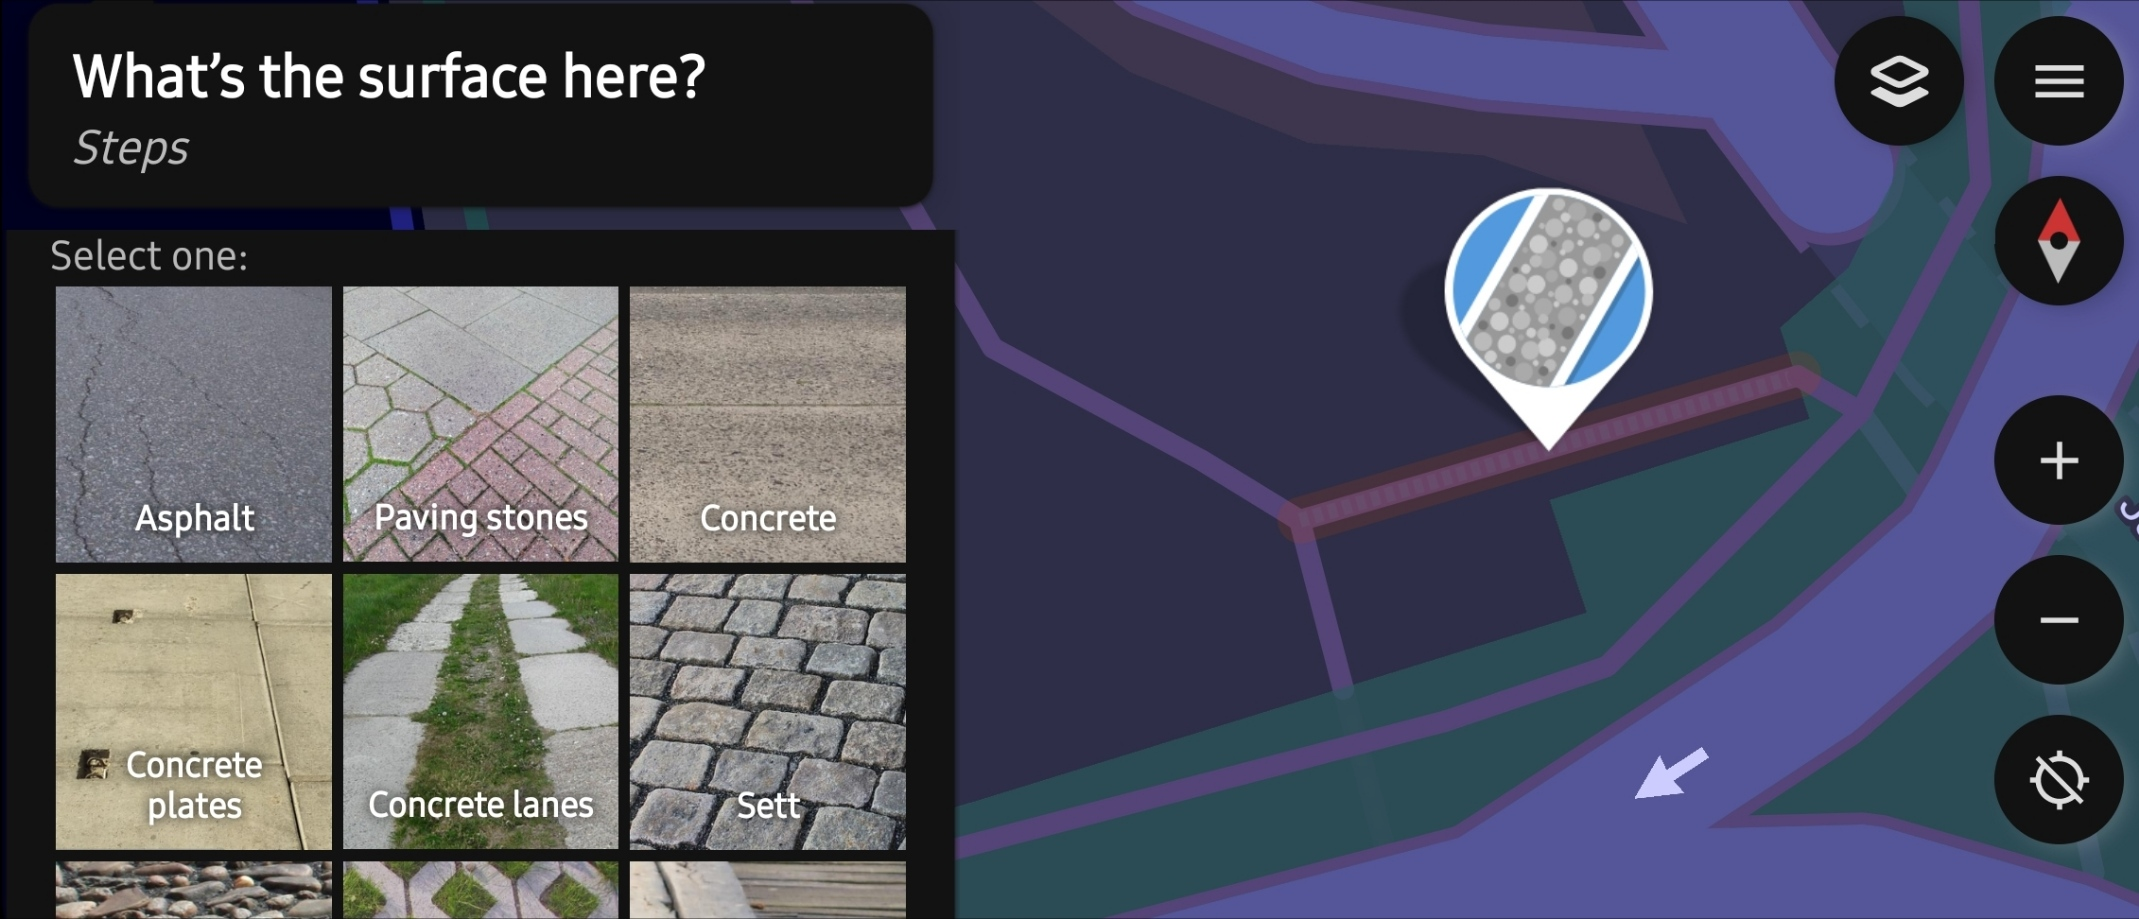
\includegraphics[width=140mm, keepaspectratio]{images/scee_example.jpg}
    \caption{A "quest" in the SCEE app, an improved version of StreetComplete; the user can submit information they see in real life \label{scee}}
\end{figure}

I also took a liking to discovering the mapping service powering most apps I use, and was interested in contributions to the dataset myself. Using it for my application would help me understand the inner workings better.

\subsection{Semantic data structure}

OpenStreetMap data is made up of elements -- nodes, ways and relations -- each describing some specific feature in space. Every element can contain multiple tags.~\cite{osmElements}

Tags are simple key-value pairs which can store strings only, but may be used to represent complicated concepts. The meaning of each key is somewhat vaguely defined and isn't standardised as there are over 96.000 different keys -- guidelines do exist, however\footnote{\url{https://wiki.openstreetmap.org/wiki/Map_features}}. Using examples, they can range from \verb|name=Tüskesátor|, defining a simple building name, to \verb|source:maxspeed=HU:zone:30|, which details speed restrictions as applicable to a given road.

The simplest element is a node. They represent objects that can not or should not be described with as a complicated surface. For instance, a bench or newsstand would be difficult to represent as anything other than points. 

A way can combine multiple nodes into a polyline, a connected chain of points. This may be used to add a building outline or a road. The accuracy can depend on the author, as there is no curve interpolation; the more sparse the contained nodes are, the more jagged the way becomes.

Relations are catch-all elements and may represent anything more complex than a single way -- in fact, they're lists of nodes and ways with metadata added through tags. A complicated building may be treated as a relation, just as an intercity bus route is a connection of highways and streets.

\subsection{Technical data structure}

Live online data is most easily queried throught the Overpass API\footnote{\url{https://wiki.openstreetmap.org/wiki/Overpass_API}}. It provides read-only access to OSM elements and accepts a wide variety of filters. The returned information is JSON-convertible, making it ideal for apps that require more control than what pre-made webmap plugins can provide.

The data may also be heavily compressed using the Protocolbuffer Binary Format (PBF\footnote{\url{https://wiki.openstreetmap.org/wiki/PBF_Format}}). On the scale of the entire planet, PBF saves over 96\% of space usage when compared to regular XML. The obvious downside is that reading this data now requires specialised libraries that can decode and uncompress it. I depended on osm4j\footnote{\url{https://github.com/topobyte/osm4j}} for this task, as it has a simple iterator to unpack elements sequentially. It's worth noting that PBF files store elements in the order of Node, Way, Relation. Earlier reads should thus be cached for later reference, only throwing away unneeded nodes as it becomes clear they're not part of any required relation -- this is analogous to how the JVM garbage collector works.

\subsection{Examples and Visualizations}

\chapter{Code structure}

I created three Gradle projects, backend, frontend and common. When building the application, the common code is compiled into both layers. Layers can thus share knowledge of the same classes, but don't need to import one another, they can be distributed as completely separate packages.

\section{Network communication}
The application was built in such a way that any current and future communication between the server and client can be made using an RFC 6455-compliant\cite{RFC6455} WebSocket provided by the server. This allows asynchronous, thread-safe communication between the two parties without being bound by packet timing. This approach also supports a "multiple clients, single server" architecture.

\subsection{Websocket usage}
Websocket communication is usually started by a client pinging a target address where a server resides. The initiating message is a handshake that must contain the host, port, resource name, and a flag showing whether the connection is secure. Secure connections must also include a TLS handshake. If the server replies, a TCP\footnote{Transmission Control Protocol, a connection-oriented protocol, used by much of today's internet traffic} connection is established -- a two-way tunnel for sending further messages with low delay. The connection has a set of possible states. There can only ever be one "connecting" socket (one that is being established but is not yet ready for data) between any given pair of machines, and sockets may fail. It's worth to keep in mind that a failed socket may drop data when disconnecting; text still in transit will not be re-sent.

Each packet, called a frame in this context, may be a data frame or a control frame. Control frames include "ping", "pong" and "close". Data frames can be used to transit text or binary data. The main noticeable difference from a standard TCP endpoint is the URI scheme: "ws://" in this case. Arbitrary data may be serialised~(see \ref{serialise}) to a data interchange format, such as JSON (JavaScript Object Notation) or YAML (Yet Another Markup Language). Text is highly compressible, so a properly set up websocket gets more efficient with larger payloads.

Websockets have several advantages applicable to this project: they're connections that are easy to keep alive and may transfer data in large batches. Setup is also easy, it's compatible with HTTP and most languages have robust libraries to manage sockets. They're slightly slower than a simple TCP connection due to their overhead; this not a problem in this case, as the ordering and timing of messages is not critical. Decoupled messages are also better for using asynchronous structures.

\subsection{Ktor-specific solutions}

In Ktor, a socket server is created by overriding the \verb|Application.configureRouting()| method. An endpoint can be made by using "webSocket" in place of an HTTP verb, such as "get" or "post"; in my case, it's available at \verb|ws://host:port/control|. The appropriate Ktor plugin must also be installed from code and can be configured here; options include the timeout and ping periods, and the selection of a content conversion strategy. I used Json with serialised class discriminators to send custom control messages. These are simple data classes in a two-level inheritance hierarchy, and replace string input validation with compile-time guarantees for the type of data transmitted.

\label{control-msg}
\begin{figure}[!ht]
    \centering
    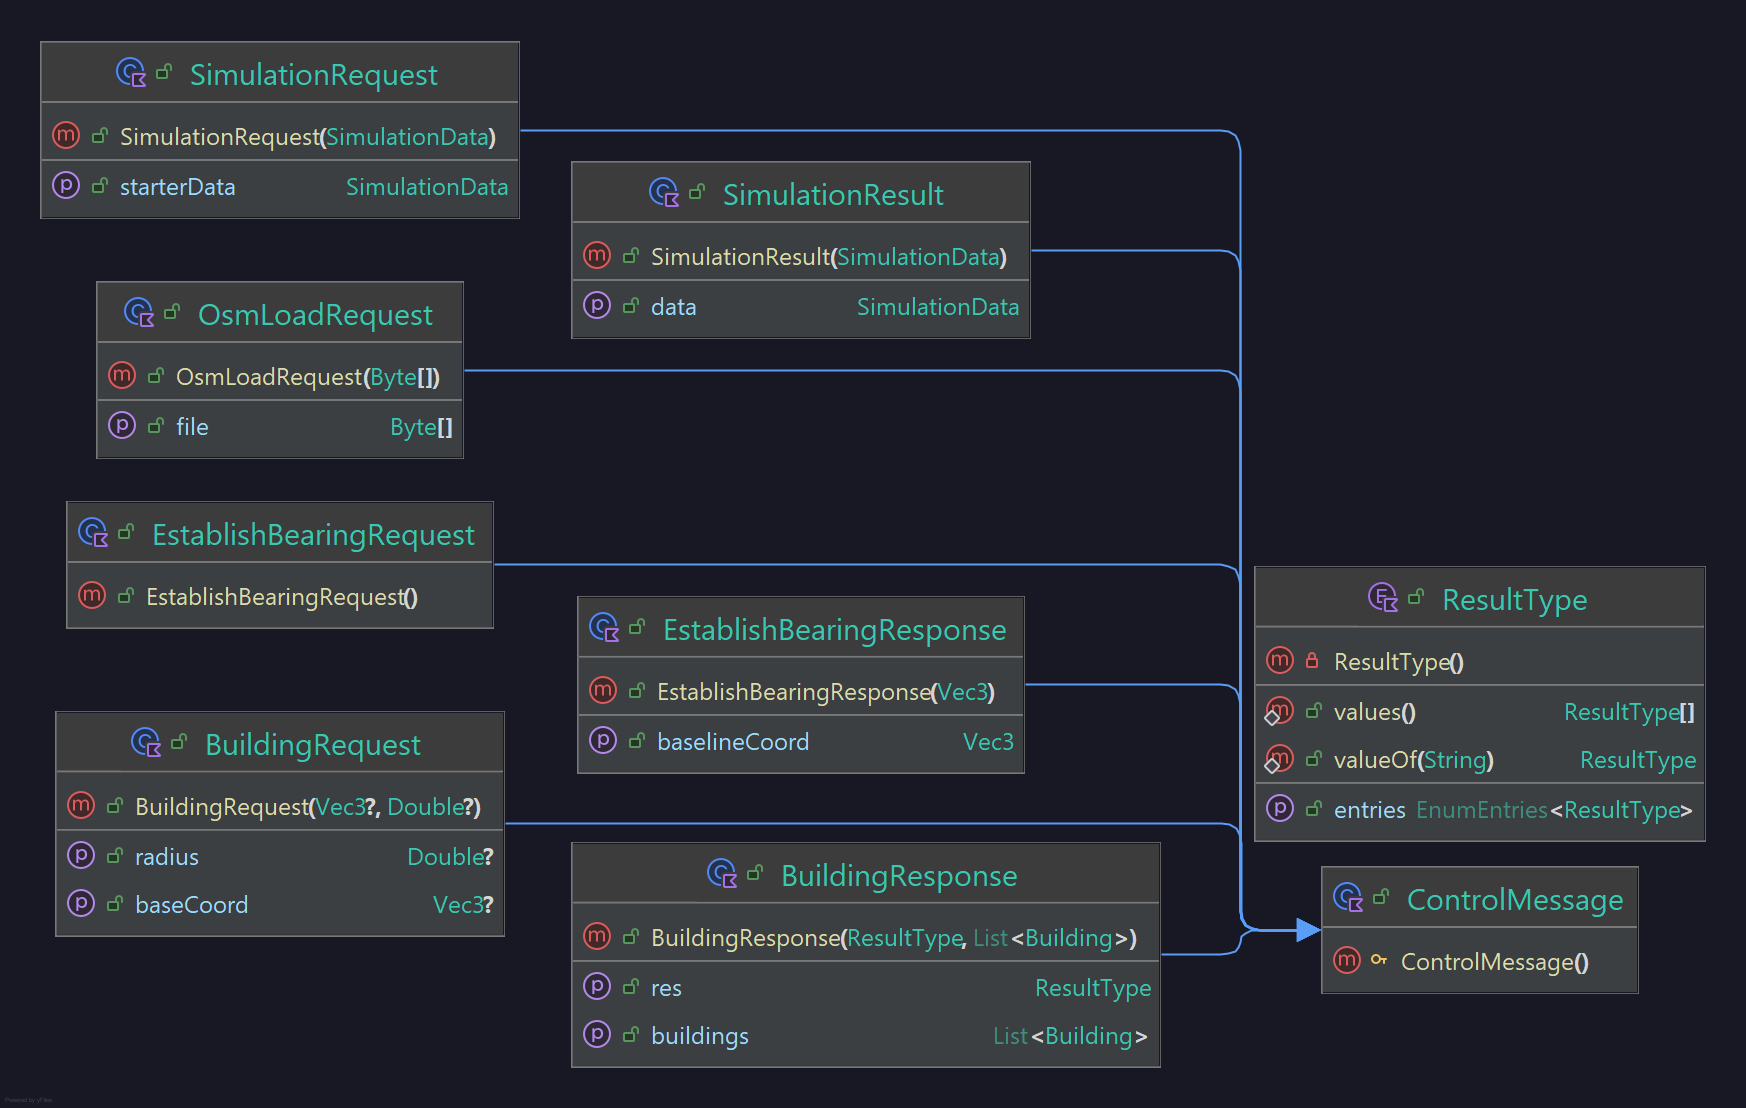
\includegraphics[width=140mm, keepaspectratio]{images/control-messages.png}
    \caption{The control messages used for communication}
\end{figure}

The endpoint has an implicit "incoming" attribute. This is a Kotlin ReceiveChannel, which is coroutine-based and helps avoid busy waiting\footnote{constantly retrying an operation (\eg~getting data from a usually empty container), this is generally wasteful} by suspending the current program flow until a message can actually be retrieved. Sending a response is done by calling \verb|sendSerialized()|, which puts data into the "outgoing" SendChannel. As long as the socket is kept open using pings, these channels may be queried continuously.

The SocketServer/SocketClient classes are responsible for the actual connections, they're treated as singletons in their respective software layers. When a message is received on either end, a map of type-function\footnote{functions are first-class citizens in Kotlin} pairs is queried, and the corresponding operation is run using a coroutine, provided it is listed. This flaunts the Open-Closed Principle in object-oriented programming, defined by Bertrand Meyer\cite{OOSC-OCP} as follows: \say{Modules should be both open and closed. [\ldots] A module is said to be closed if it is available for use by other modules. This assumes that the module has been given a well-defined, stable description.} While the message class itself is open to extension, any modification requires changing the list of callback functions. I found this to be an acceptable trade-off, as it protects against typos, missing fields and the processing of unknown messages.
The server keeps a list of all connected clients and treats them as subscribers, sending every response to all of them; one backend instance can service multiple clients.

\label{file-upload}
The client may send a protocol buffer file through the \verb|/pbf_file| POST endpoint to overwrite the current database with a different region of the globe. Data is loaded as described in section~\ref{pbf-loading}. This is the single message that does not use websockets for transmission.

\section{The database}

I chose SQLite as my database engine. It's lightweight, decently fast, and self-contained. The theory is that the .db file may be used like a video game save if needed, since deep copies can be mode by duplicating the file. Most other database engines are unsuitable for this, because their data may span multiple files or even systems. SQLite has no automatic backups -- losing this program's database is not a concern, though, as it can be rebuilt in seconds. For transactions, the standard ACID (atomicity, consistency, isolation, durability) principles are followed.

\label{pbf-loading}
The database is created when loading a new PBF dataset, and can be read unlimited times until a new file is presented. The program spawns a PBF iterator from the osm4j library and reads every element into an OsmStorage object. Nodes and ways are read unconditionally, as relations must reference them to hold any meaningful data. Out of every category, elements with the \verb|highway| or \verb|building| tag are collected, their child elements retrieved and dumped into the database. After this process, the on-CPU storage object is purposefully thrown away and cleaned up due to the high number of unused nodes.

I ended up going with a very simple data structure of just two tables, Buildings and Roads. Both tables have osm\_id, tags and ways columns, and buildings include additional information about their location, OSM element type, as well as a capacity, calculated as a function of their area and height. Some buildings have a "height" tag that's specified in meters, or a "levels" tag counting its floors. If none of these is present, I calculate the value as if there was only one storey. Capacity is used by the random selection algorithm while simulating to weigh the options. Roads are stored as simple splines of one or more serialised ways, with their separate tags also stored (if they have any). This does not encode width information as per OSM guidelines.

The OSM tags take up the most space in the database, as they're simple strings that can't be reasonably simplified. Since the key-value pairs are unique most of the time, I found no real gains in creating a foreign key structure for them and instead used a JSON serialiser. Later editions of the software could have a hybrid solution: a lookup table for common values, and simple string storage for all others.

\subsection{Data access}

Database communication is handled by the DatabaseAccess singleton. All methods are independent of the engine being used, so the database connection string could be swapped to use any other engine supported by Exposed. Queries are serialisable transactions, which mostly prevents read-write collisions in case the user requests to load a new dataset while the current one is still being queried. Kotlin natively supports Sequences, a list type that can produce items while it's being iterated. I made use of this to send building data to the socket in smaller chunks, before the whole transaction is done, reducing crashes and improving performance. Exposed provides a DSL-specific transaction block, which runs all contained code in a database context, automatically dropping changes if any errors are raised. If the transaction block would ever freeze, incomplete data may be sent, but the program does not have to terminate.

\section{Common classes}

I made the following utility classes in the common project. \begin{itemize}
    \item \textbf{SerializeableNode/Way/Tag} -- Data classes explicitly annotated as @Serializable for Ktor, they wrap their respective osm4j types. Tags are expressed as "key=value" strings.
    \item \textbf{Vec3} -- A three-dimensional vector class with basic arithmetic methods, and Doubles instead of Floats. These are used throughout the program to maintain higher precision when using real-world coordinates.
    \item \textbf{Building, Road} -- The runtime equivalents of the database records. The frontend can't see the database structure, only these representations. They also function as Data Access Objects (DAOs) for Exposed.
    \item \textbf{Agent} -- A person in the city and simulation. They have a pre-set speed and age group. Their precise location in the world is also stored.
    \item \textbf{ObservableMap} -- A typical Kotlin MutableMap, extended with callbacks for any changes that occur (for example, adding an item).
    \item \textbf{ControlMessage (and inheriting classes)} -- A simple explicitly serialisable class with predefined fields; this is how I ensured that every websocket message contained the expected data. See \ref{control-msg}
\end{itemize}

\label{serialise}
Exposed supports custom columns, which I used to convert each Vec3 instances to a VARCHAR\footnote{variable length character array, it can store arbitrary text up to its length limit, only using the necessary number of bytes} type in SQL. This is type-safe when reading or writing, conversion happens automatically.
\begin{lstlisting}[caption=Custom column type in JetBrains Exposed]
    object Vec3ColumnType : ColumnType<Vec3>() {
    override fun sqlType(): String = "VARCHAR(50)"
    override fun valueFromDB(value: Any): Vec3 {
        return when (value) {
            is String -> Vec3.fromString(value)
            else -> ...}} ... }
\end{lstlisting}

\section{The frontend}

\begin{figure}[!ht]
    \centering
    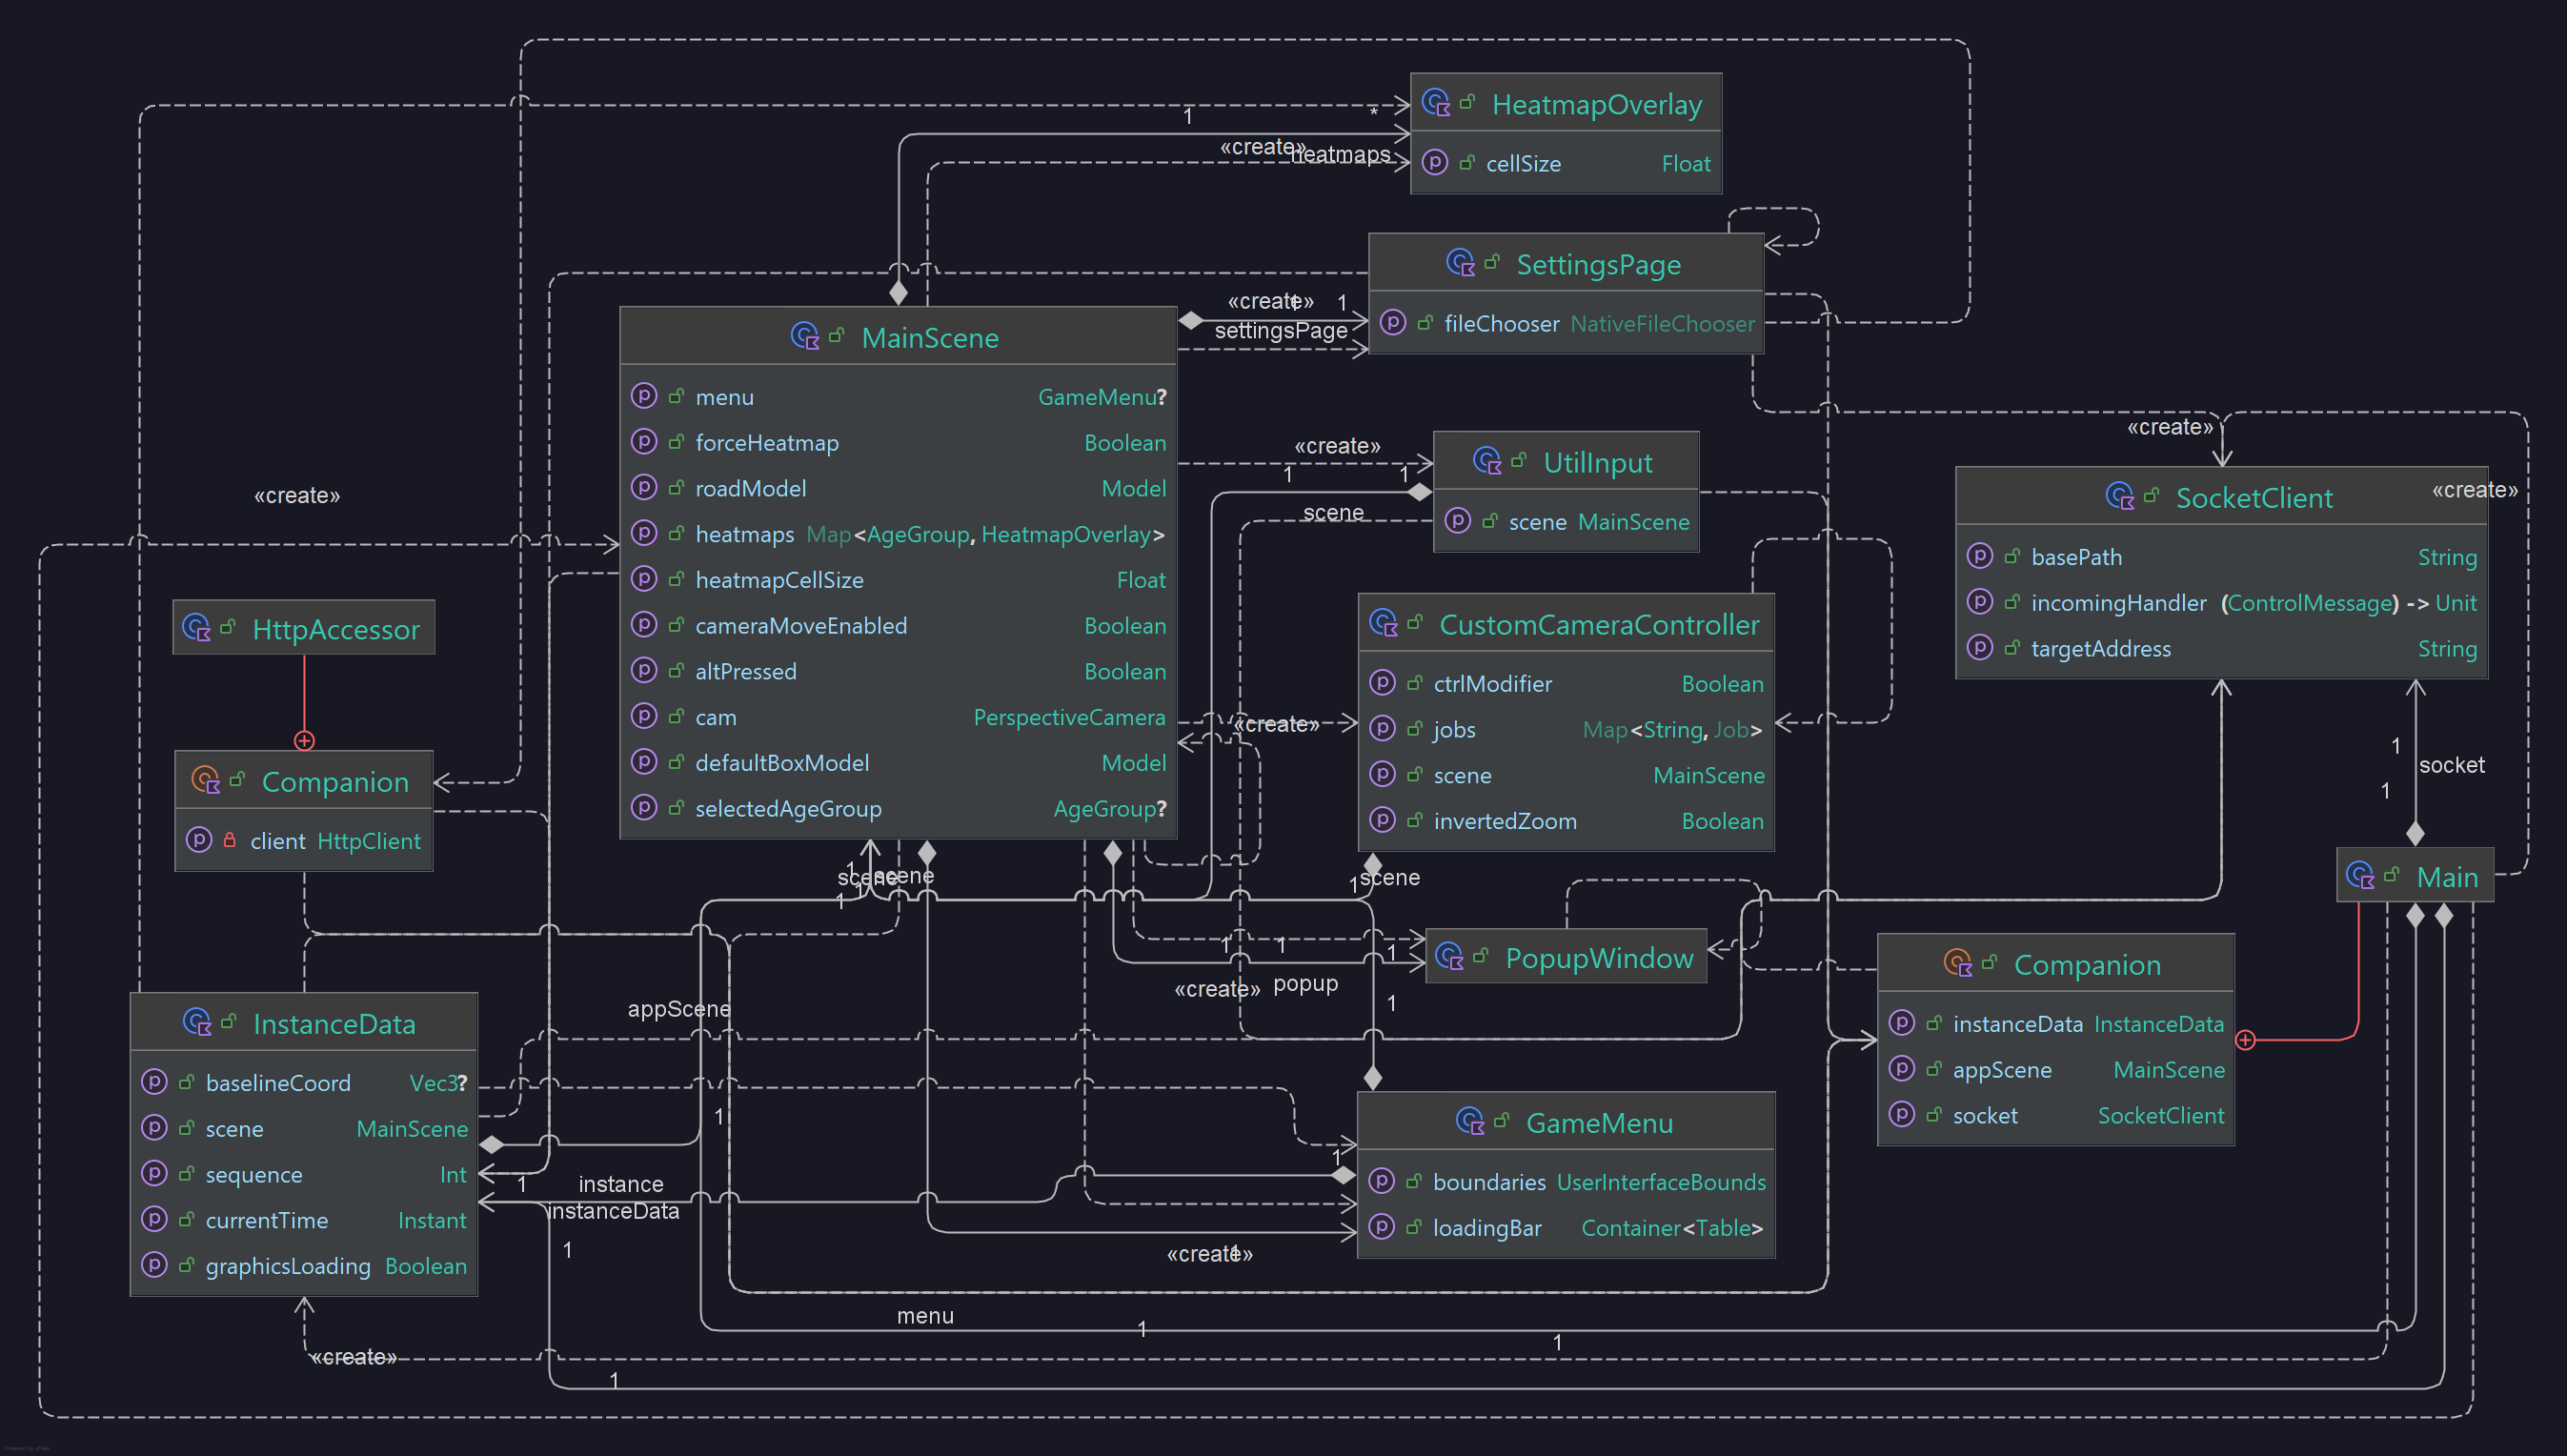
\includegraphics[width=140mm, keepaspectratio]{images/frontend-classes.png}
    \caption{Diagram of the most important classes on the frontend}
\end{figure}

The client project takes a slightly more centralised approach. It's a libGDX application, with a \verb|MainScene| class as the focus. Input controllers and other data are imported directly into this class. LibGDX variables utilise Kotlin's lateinit feature as they can only be assigned once there is a current graphics context, in the \verb|create()| function.

The \verb|InstanceData| class handles everything not directly related to graphics and OpenGL functions; it orchestrates requests, handles incoming messages, gives commands to the main scene and its menus. All queried objects are put into an ObservableMap, and puts automatically trigger the corresponding function to insert the object into the scene.

%TODO
\chapter{Simulation}

The frontend can be quite interesting as just a way to survey a city from a bird's eye view. The program's real use lies in data analysis, though. Over the semester, I tried multiple approaches for creating an agent-based simulation, with all but the last attempt failing due to technical circumstances.

\section{Deprecated versions}

The first concept was very simple. Each agent would pick a two random buildings as start and end points, and would travel between them in a straight line, with constant speed. Actors would be shown in the graphical scene as individual cubes, moving in small increments. The backend simulated movement in one minute steps, and after each one, the modified agents would be collected and sent over the websocket in multiple chunks, so as to reduce the chances of overloading the socket. The problem here was one of scalability. Fifty or a hundred agents could easily be processed and shown in real time, but that obviously was not enough to draw any meaningful conclusions about behaviour. Displaying more agents caused a simply unacceptable framerate of three frames per second. Although I used the same visual model for every agent, batching and caching could not be used due to the chaotic nature of their overall movement. The design is visible in the appendix,~\ref{overlay_v1}

The second version improved performance by processing the agent updates non-visually and dividing up the playfield into relatively small chunks to act as a heatmap; it was a separately renderable on top of the main scene. Each update's coordinates were fed into the overlay, and an opacity value was calculated for every chunk. The result was a serviceable tool that, while updating constantly, still had bad performance. A new object cache was being created every time I opened the heatmap UI, and this taxed the rendering thread heavily. However, once all updates have been processed, the performance was decent. This gave me the idea of running full simulations as fast as possible, and only transferring the final values over the socket. This design is also in the appendix,~\ref{overlay_v2}

\label{simulation-working}
\section{The working implementation}

I ended up keeping the agent idea, but focused on the need for the frontend to be uninvolved aside from requesting and displaying content. As such, the server only recognises its own spatial scale and the heatmap's chunk size needs to be converted. The client can choose time constraints and an agent count for the simulation, using fields in the dialog opened by the "play" button on the frontend.

The server starts each simulation from scratch by copying the HeatmapData instance sent by the client. The requested number of agents is randomly distributed on the map, with the buildings chosen from the database, weighted by the "capacity" column: a large residential building is more likely to have agents start there than a small boutique. Each person can then choose a target building every minute, but may also choose to remain where they are. With a resolution of 7.5 simulated seconds, the difference between the goal and the current location is determined, normalised, and the agent is nudged along by adding this value to its position multiplied by the agent's speed. As of now, the speed is pre-determined in the Agent class, intended as a placeholder for different vehicle types.

The simulation constantly the copied instance, adding one to the value of the cell that contains the current step. The grid size is received in degrees of latitude/longitude. The correct cell's id is calculated by flooring the coordinates using the baseline and grid size. The map is not pre-allocated, the desired cell is created on the fly if it does not exist -- this reduces data transfer significantly. Updates are grouped by minute and then by agent. Once the terminal state is reached, a SimulationResult message is sent back with the heatmap cells.

The data is transformed by the client, scaling the coordinates contained in each cell's identifier back, and placing each integer into the correct slot of the libGDX heatmap. Every value is absolute, scaling is done at render time.
\begin{figure}[h]
    \centering
    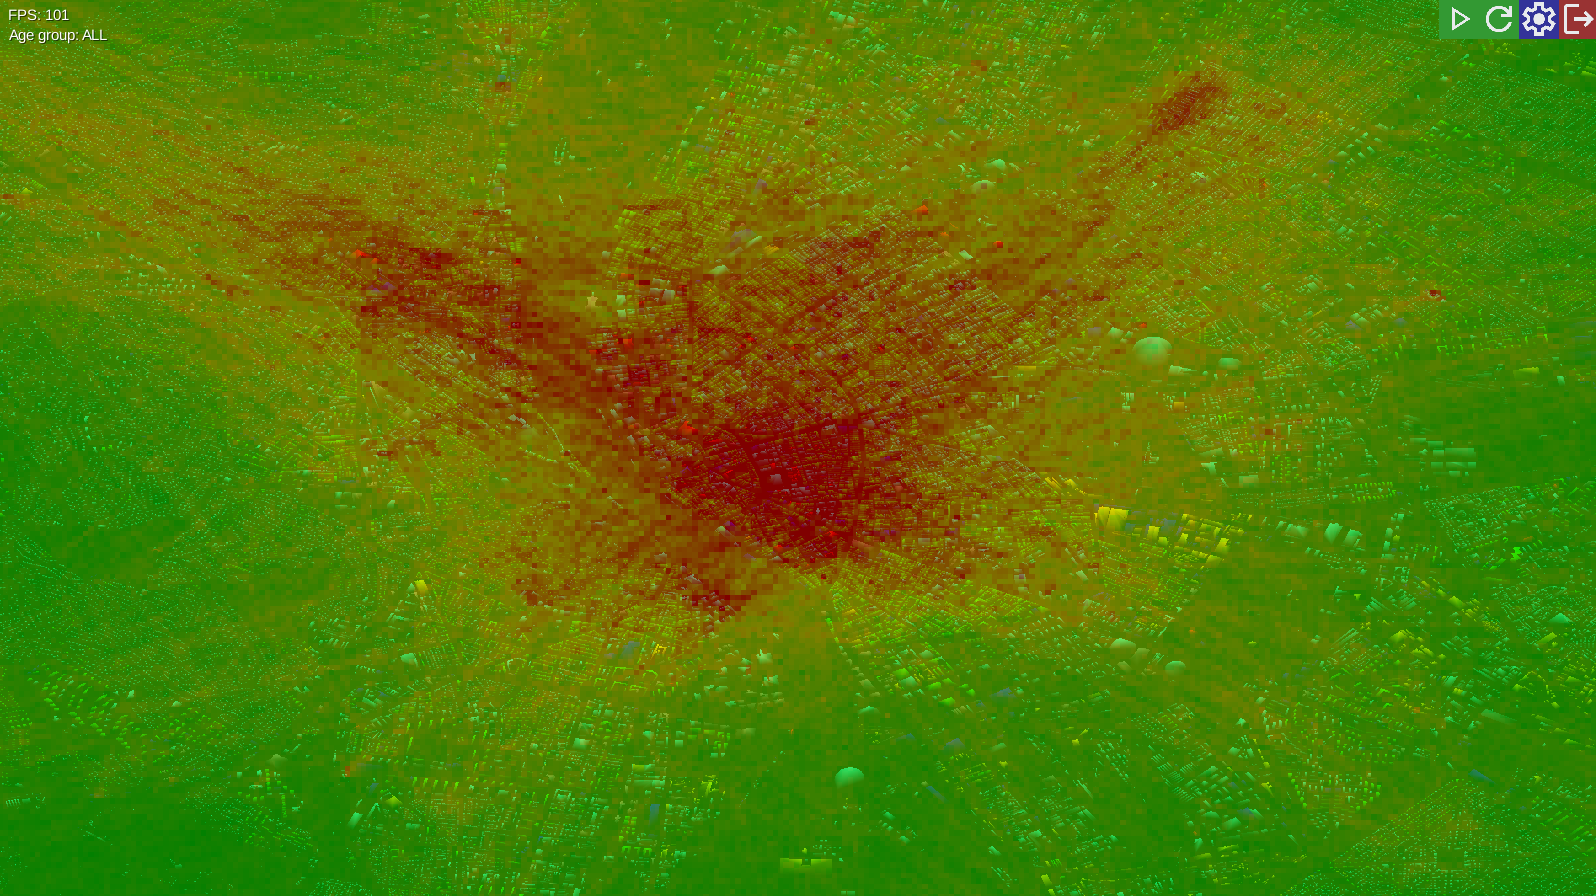
\includegraphics[width=140mm, keepaspectratio]{images/overlay_v3.png}
    \caption{A shaded overlay, showing most common agent paths; this version ended up in the program\ \label{overlay_v3}}
\end{figure}

\subsection{Building selection logic}

People in the simulation choose targets based on a simplified statistical model. They may be in one of four primary age groups: children, teens, adults or the elderly. Time of day, age group and building type can be represented as a three-dimensional distribution. Some building types (such as schools) are visited rarely at night, but very often in mornings. Age group and building type is connected as well: children are generally not expected to travel to industrial complexes.

I represented this as two static distributions, stored on the server's side. Agents first decide if they want to travel at all, this happens 25\% of the time overall, split up into two checks. The chance of a given agent travelling to a certain building type is calculated by multiplying the time-type and age-type values together. Each product is the probability of travelling to the given building type; agents pick a random type that has a chance between 0 and a randomly selected floating point value, up to 1. If the calculated building variety is the same as the current building, the agent does not leave; otherwise, a random building is picked, the likelihood of any individual target is decreases with distance. The process maintains a pool of buildings to pick from. When an item is selected, it's removed from the cache. If the cache has no buildings of the selected type, a request is made to the database for that type.

The method thus has three random variables. This requires many more agents than a more sophisticated model to achieve the expected distribution, but its accuracy is acceptable, provided the required processing power is available. Since the model is based on individual decisions, expansion is not too difficult -- more variables can be added as needed. 

I took inspiration from the video game Cities: Skylines II for the simulation system. There, pathfinding is based on time, comfort, money and individual citizen behaviour.\cite{CSII-traffic} The most important takeaway was the differing needs of certain age groups. As comfort and money was not applicable, I instead differentiated agent behaviour by the type of buildings they would visit at certain hours of the day. Travel time is a linear function of the distance covered and not influenced by road geometry. This was overall a computationally cheap and easier to implement solution, and it still provided specific patterns for the four age groups.
%----------------------------------------------------------------------------
\chapter{Presentation layer}

\section{Low level graphical challenges}

By using near-machine graphical interfaces, we lose certain simplified operations, for instance the ability to draw complex three-dimensional shapes directly from code. Most graphics cards have certain predispositions about the data they process, and in low-level cases, our program can't guarantee that those rules will be followed. LibGDX provides strong foundations in place of ready-made solutions, which the developer can use to implement or in some cases, disregard the GPU's written or unwritten requests. These include the following examples.
% A gépközeli grafikai interfészek használatával elveszítünk bizonyos egyszerűsített műveleteket, például a komplex alakzatok kódból történő közvetlen felrajzolását. A legtöbb grafikus kártya bizonyos feltételezésekkel él a rajta átfutó adatok feldolgozásakor, és így ezek teljesülésére sem képes garanciát vállalni a programunk. A libGDX kész megoldások helyett erős alapokat biztosít, amivel a fejlesztő saját döntése szerint implementálhatja vagy eseti alapon figyelmen kívül hagyhatja a GPU írott-íratlan igényeit; pár példát bemutatok ezekből.

\subsection{Triangulation, ear-clipping algorithm}

Triangles are the most commonly used basic two-dimensional shape that is supported without too many caveats on all platforms. Therefore, it's advisable to reduce any displayed models to a group of them.
%A két dimenziós háromszög a leggyakoribb elemi alakzat, amit minden platform grafikus interfésze feltétel nélkül támogat; célszerű lenne tehát a modelleket ezek összességére redukálni.

One geometrically intuitive division operation is the ear-clipping algorithm. An ear is defined as a triangle made up of three successive vertices of a polygon, where the middle vertex is convex -- in that point, the shape's inner angle must not exceed 180 degrees ($\pi$ raidans).\cite{TriangulationByEarClipping} Areas defined by such triples are guaranteed to be subtractable from the polygon's area, since by definition, they can not contain any holes, removing the need to compensate for empty space. The action can then be repeated on the remaining area, each successive step will result in a new triangular piece; when only three vertices remain, we have achieved our goal of subdivision.
% Geometriailag intuitív felosztó eljárás a fülvágó algoritmus (ear-clipping algorithm). Fül alatt olyan háromszöget értünk, amit egy poligon egymást követő három csúcspontja alkot, melyek közül a középső konvex -- tehát az adott pontban a sokszög belső szöge legfeljebb 180 fok ($\pi$ radián).\cite{TriangulationByEarClipping} Az ilyen hármasok által határolt terület garantáltan kivonható a poligonéból, mivel definíció szerint nem lehet lyuk vagy kihagyás benne, így nem kell kompenzálni az üres térért. Az eljárás a megmaradt területre megismételhető, és minden lépés egy újabb háromszög alakú részletet fog eredményezni; így a célunkat el is érjük, amikor már mindössze három csúcspont marad.

The goal of this algorithm is to create a list of vertex indices that should be connected into triangles, in order to cover the original polygon fully and efficiently. As a useful side effect, this makes calculating the mathematical area trivial as well.
% Az algoritmus célja tehát a fent leírt módszerrel kiszámítani, hogy egy tetszőleges sokszög lefedéséhez milyen módon kell háromszögekké összekötni a kapott vertexeket. Hasznos mellékhatás, hogy ezzel a sokszög területének összegzése is triviálissá válik.

In the case of libGDX, the EarClippingTriangulator class takes care of this common use case. Following OpenGL idioms, the relevant function requests floating point values (vectors decomposed into their axes), and it results in a list of whole number indices -- every group of three defines a triangle to be created.
%A libGDX esetében a gyakran visszatérő felhasználásnak köszönhetően külön osztály gondoskodik erről (EarClippingTriangulator). Az OpenGL idiómáinak megfelelően lebegőpontos értékekre bontott vektorokat kér bemenetként, eredménye pedig egy egyszerű, indexekből álló lista -- ennek elemei hármasával határoznak meg egy háromszöget.

\begin{lstlisting}[caption=Example usage of the EarClippingTriangulator class]
    val floats = baseNodes.flatMap { listOf(it.x, it.z) }.toFloatArray()
    val triangles: ShortArray
    val triangulator = EarClippingTriangulator()
    triangles = triangulator.computeTriangles(floats)
\end{lstlisting}

\subsection{Winding order}

Many graphical effects - including lighting - require knowledge of the affected faces' normal vectors. In the mathematical sense, this means a direction which is perpendicular to the whole surface, when applied to any contained point of it. %TODO meh 
When observing the side from this particular direction (the vector between the camera and a given point of the face can be represented as a multiple of the normal), the apparent size is at its largest -- in layman's terms, we're seeing the front without any rotations around axes that don't match the normal.% Számos effektus, például megvilágítás alkalmazásához szükséges ismerni az érintett lapok normálvektorát. Matematikai értelemben ez olyan irányt jelent, ami egy felület tetszőleges pontjában merőleges a teljes felületre. Ebből az irányból nézve a felület látszólagos mérete a lehető legnagyobb, mivel köznyelvileg "szemből" látjuk a sokszöget, egyik irányba sincs elforgatva.

The visibility of a polygon can technically also be treated as an effect. To reduce the number of draw calls, it's advisable to only handle faces that have their intended front side visible from the camera's perspective. By default, OpenGL utilises "back-face culling": the spectator can only see shapes where the order of vertices is counter-clockwise (when plotted in relation to the vector connecting the viewpoint and the weighted center of the polygon). This behaviour is modifiable as follows.
%Grafikai hatásnak tekinthető az is, hogy egyáltalán látható-e egy poligon. A kirajzolási műveletek számának csökkentése miatt célszerű csak azokat a lapokat számba venni, amiknek a kívánt oldala mutat a kamera felé. Az OpenGL alapértelmezetten "back-face culling" elven működik: a néző csak azokat az alakzatokat látja, amiknek a nézőpontot és az alakzat középpontját összekötő vektor körüli vertex-sorrendje az óramutató járásával ellentétes. Ez a viselkedés az alábbiak szerint módosítható.

\begin{lstlisting}[caption=Example for changing OpenGL's culling properties through libGDX]
    Gdx.gl.glEnable(GL40.GL_CULL_FACE) //enabling
    Gdx.gl.glCullFace(GL40.GL_BACK) //setting filtered side (rear)
    Gdx.gl.glFront(GL40.CW) //changing the intended winding order to clockwise
\end{lstlisting}

\subsection{Using the main thread}

In contrast to the project's simulation module, the user interface is difficult to parallelise. OpenGL functions are usually not thread-safe, requesting and modifying a single graphical context from multiple areas of code is dangerous and will often lead to crashes.

%A projekt szimulációs részével szemben a megjelenítés nehezen párhuzamosítható. Az OpenGL műveletek általában nem szálbiztosak, egy grafikai kontextust egy időben több helyről használni és módosítani nem érdemes; programunk futása hamar hibára fut.

The graphics library abstracts communication with the operating system and GPU as much as possible. In return it's the developer's responsibility to reduce GPU calls to the absolutely necessary amount. While unique calls are being processed, the GPU can't pass newly created frames to the processor, which is visible as the screen 'freezing' -- this is easily observable in the chapter dedicated to performance. 

%A grafikus könyvtár a lehető legjobban elrejti az operációs rendszerrel és GPU-val történő kommunikációt, cserébe viszont a fejlesztőnek ügyelnie kell arra, hogy az abszolút szükséges mennyiségre csökkentse a GPU hívásokat. Amíg egyedi kérések feldolgozása történik, a kártya nem tud újabb képkockákat átadni a processzornak, a monitoron tehát "megfagy" az animáció -- ez a későbbi, teljesítményt taglaló fejezetben jól látható.

Aside from frame construction, the program only uses the main graphical thread for creating unique models for each building, as this can't reasonably be done on the CPU. I decided against a complex thread-scheduling solution, as the GPU  only receives a heavy workload when creating a new save, or loading an OSM buffer file. When programming, I only had to built on available tools; I used a simple lambda function to obtain the main thread context when needed.

%A programban a fő szálat egyetlen helyen használom jelentősen a képalkotást leszámítva. A vonalakkal meghatározott épületek egyedi modelljét csak a GPU képes legyártani. A végső szoftverben a szálhasználat ütemezése helyett szokásosnak mondható módon betöltő-képernyő jelenik meg új mentés vagy adatcsomag előkészítése közben. Programozási szempontból csupán a meglévő eszköztárra kellett építenem, lambda függvényt készítettem a fő szál kontextusának tetszőleges szálon történő megszerzéséhez.

\begin{lstlisting}[caption=Helper function for getting the draw thread]
private suspend fun <T> runOnRenderThread(block: () -> T): T {
        return suspendCoroutine { continuation ->
            Gdx.app.postRunnable {
                continuation.resume(block())
            }
        }
    }
\end{lstlisting}

\section{Implementation}
The program's visual part can be divided into modules. Aside from the interactive, three-dimensional OpenGL scene showcasing the buildings, there exist multiple independent components, aiding user communication.

%A program grafikus része modulokra bontható. Az épületek bemutatására hivatott interaktív, három dimenziós OpenGL teret csomagoló, főszerepű jeleneten kívül több független, felhasználói kommunikációt megvalósító komponens is létezik.

\section{The main scene}
Buildings are presented in a simplified manner, ignoring any vertical terrain changes. Stylistically, it was inspired by contemporary city building video games (such as SimCity and Cities: Skylines), as well Google Earth.

%A grafikus felület egyszerűsített, domborzatot figyelmen kívül hagyó módon ábrázolja az egyes épületeket. Stílusa inspirációt merít a kortárs városépítő videojátékok (SimCity, Cities: Skylines) és a Google Earth kinézetéből. %TODO: felülnézet?
\begin{figure}[!ht]
    \centering
    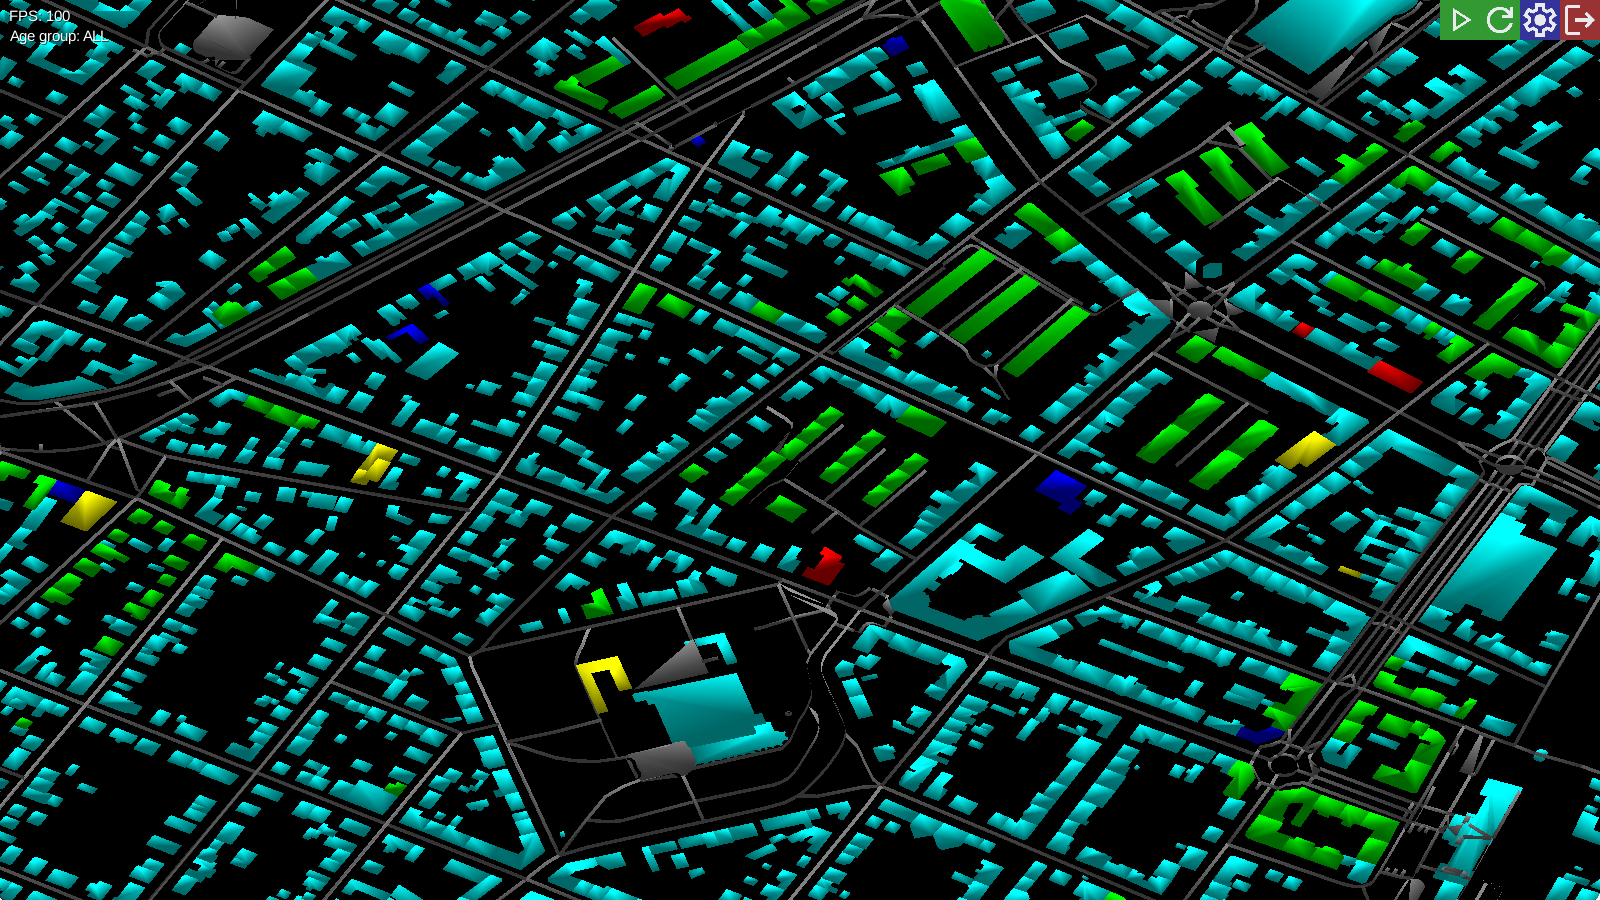
\includegraphics[width=150mm, keepaspectratio]{images/main_graphics_view.png}
    \caption{The main page of the app, with a "false 3D" view}
\end{figure}

\subsection{Custom camera control}

A libGDX jelenetei egyetlen bemenetet feldolgozó adapter objektumot, vagy azok összességéből készült multiplexert képesek tárolni. A könyvtár készítői által ajánlott alapértelmezett 3D keretprogram\cite{basic3DlibGDX} a CameraInputController osztályt használja; ez az eseménykezelő az egérrel végzett forgatást és nagyítást adja hozzá az azt meghívó jelenetnek.
A publikus InputAdapter interfészre támaszkodva saját kamera- illetve menüfunkciókat fejlesztettem. A megtekintési szög zárolva van, a felhasználó rögzített felülnézetből vizsgálhatja a backend adataiból készült képet. A mozgatás kihasználja a kamera képkockánként szükséges frissítését. A navigációs gombok megnyomása bizonyos mennyiséget hozzáad a jelenlegi a célmozgáshoz, és ez a mérőszám képkockánként százalékosan csökken, ahogy a kamera halad. A számláló kellően kicsi értéke mellett a mozgás azonnal befejeződik.
Ennek eredménye egy jól kinéző sebességkezelés, ami elkerüli a robotikus, hirtelen irányváltozásokat. Mivel egyszerre több parancs végrehajtása is történhet, minden, a kamera állapotát változtató függvény mutex\footnote{mutual exclusivity} zár alá esik; enélkül a képkockák kirajzolása közben ütköző lépések a képernyő ugrálását idéznék elő.
% TODO code section

\
 Egy komplexum, de akár az azt határoló vonalak által leírt poligon is lehet konkáv, így a teljes modellek felépítéséhez a fülvágó algoritmust használtam.

A backend-ről származó adatokból természetesen nem csak az entitások pozíciója, formája lényeges, az OpenStreetMap adathalmaz alapján csoportosíthatók és színezhetők  

\chapter{Testing and deployment}

As the app's communication does not follow typical REST patterns, I used a combination of end-to-end\footnote{real use cases are performed in the app and the output is checked} and performance tests.
Machine 1 is a Windows 11 desktop computer with an AMD Ryzen 5 7600X processor, 32GB of RAM and an AMD Radeon RX 6750 XT GPU. It is connected to the internet via 1Gbps Ethernet. Machine 2 is a laptop running Arch Linux with an AMD Ryzen 5 7520U CPU, 16GB of memory, and integrated AMD Radeon graphics. During the tests, the laptop used 5GHz Wi-Fi with an approximate speed of x/y Mbps (download/upload). In all instances, the program was started using Gradle and Oracle OpenJDK version 23.x.x. Containerisation was not used during testing.

\section{End-to-end testing}
%TODO: runtime comparisons with few or many agents
%TODO: testing of correctness: distribution should match expectation
%TODO: docker container %CONSIDERED DONE
\chapter{Further avenues of development}

While the program is already capable of providing good insights into many cities' basic travel patterns, it may be improved in the future in multiple ways. These include:
\begin{itemize}
    \item a more robust networking system, capable of efficiently handling dropped packets and service disruptions -- this would require a medium-to-large scale refactoring of the code, and is feasible if any of the other features are implemented
    \item the addition of roads to the simulation model, making agents travel along these known good paths instead of the "as the crow flies" method
    \item different modes of transportation, including walking, car use and public transit
    \item adding real public transit lines with vehicles 
    \item interactive map with the ability to move and delete buildings or other objects
    \item general optimisations
\end{itemize} %CONSIDERED DONE



% List of Figures, Tables
%~~~~~~~~~~~~~~~~~~~~~~~~~~~~~~~~~~~~~~~~~~~~~~~~~~~~~~~~~~~~~~~~~~~~~~~~~~~~~~~~~~~~~~
%\listoffigures\addcontentsline{toc}{chapter}{\listfigurename}
%\listoftables\addcontentsline{toc}{chapter}{\listtablename}


% Bibliography
%~~~~~~~~~~~~~~~~~~~~~~~~~~~~~~~~~~~~~~~~~~~~~~~~~~~~~~~~~~~~~~~~~~~~~~~~~~~~~~~~~~~~~~
\addcontentsline{toc}{chapter}{\bibname}
\bibliography{bib/mybib}


% Appendix
%~~~~~~~~~~~~~~~~~~~~~~~~~~~~~~~~~~~~~~~~~~~~~~~~~~~~~~~~~~~~~~~~~~~~~~~~~~~~~~~~~~~~~~
%----------------------------------------------------------------------------
\appendix
%----------------------------------------------------------------------------
\setcounter{chapter}{\appendixnumber}
%\setcounter{equation}{0} % a fofejezet-szamlalo az angol ABC 6. betuje (F) lesz
\numberwithin{equation}{section}
\numberwithin{figure}{section}
\numberwithin{lstlisting}{section}
%\numberwithin{tabular}{section}

\chapter{Heatmap designs}

\stepcounter{section}
\begin{figure}[!h]
    \centering
    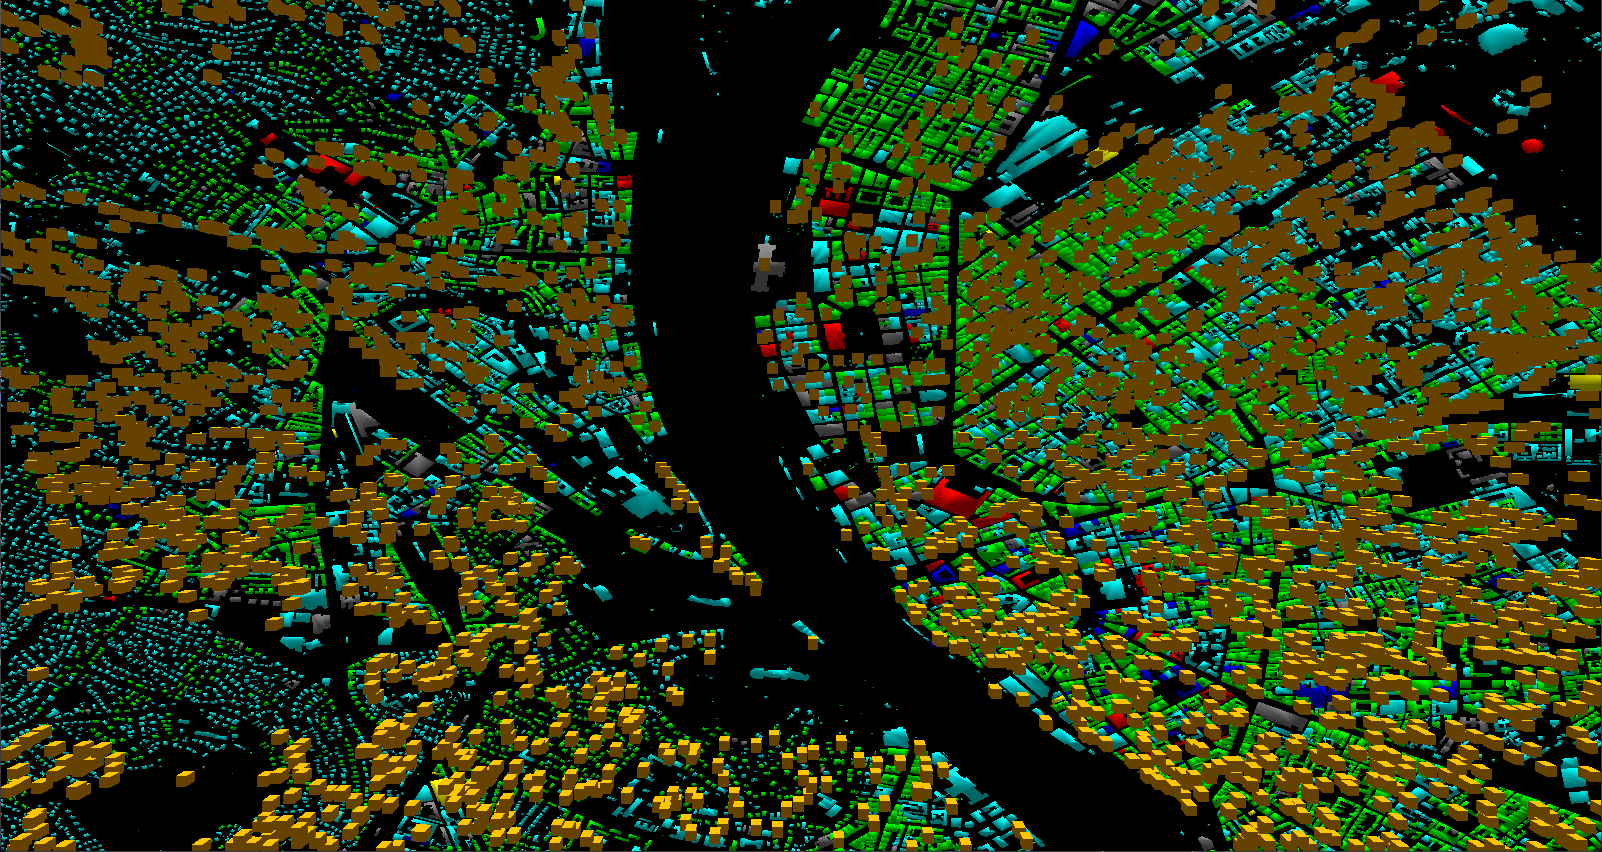
\includegraphics[width=110mm, keepaspectratio]{images/overlay_v1.png}
    \caption{An array of cubes displayed over the city of Budapest, each representing an agent; this was the first overlay version\ \label{overlay_v1}}
\end{figure}
\begin{figure}[!h]
    \centering
    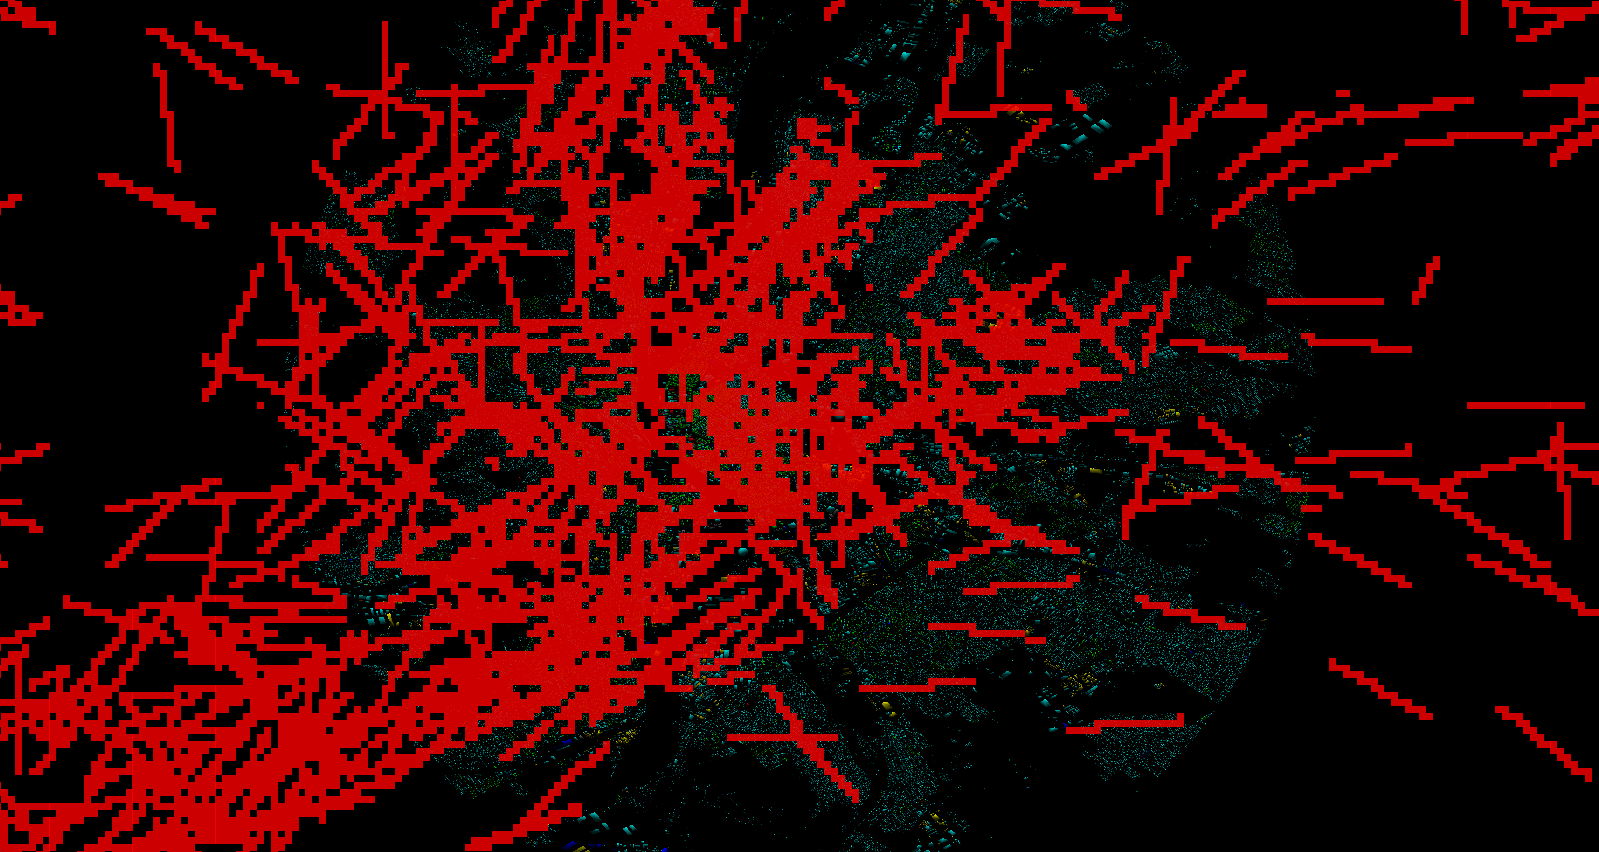
\includegraphics[width=110mm, keepaspectratio]{images/overlay_v2.png}
    \caption{An overlay with flattened opacity, displayed over the city of Budapest. Agent paths are randomised and are traversed in a straight line; this was the second overlay version\ \label{overlay_v2}}
\end{figure}

\label{comparison_heatmap}
\chapter{Agent count and age group comparison}

\stepcounter{section}
\begin{figure}[!h]
    \centering
    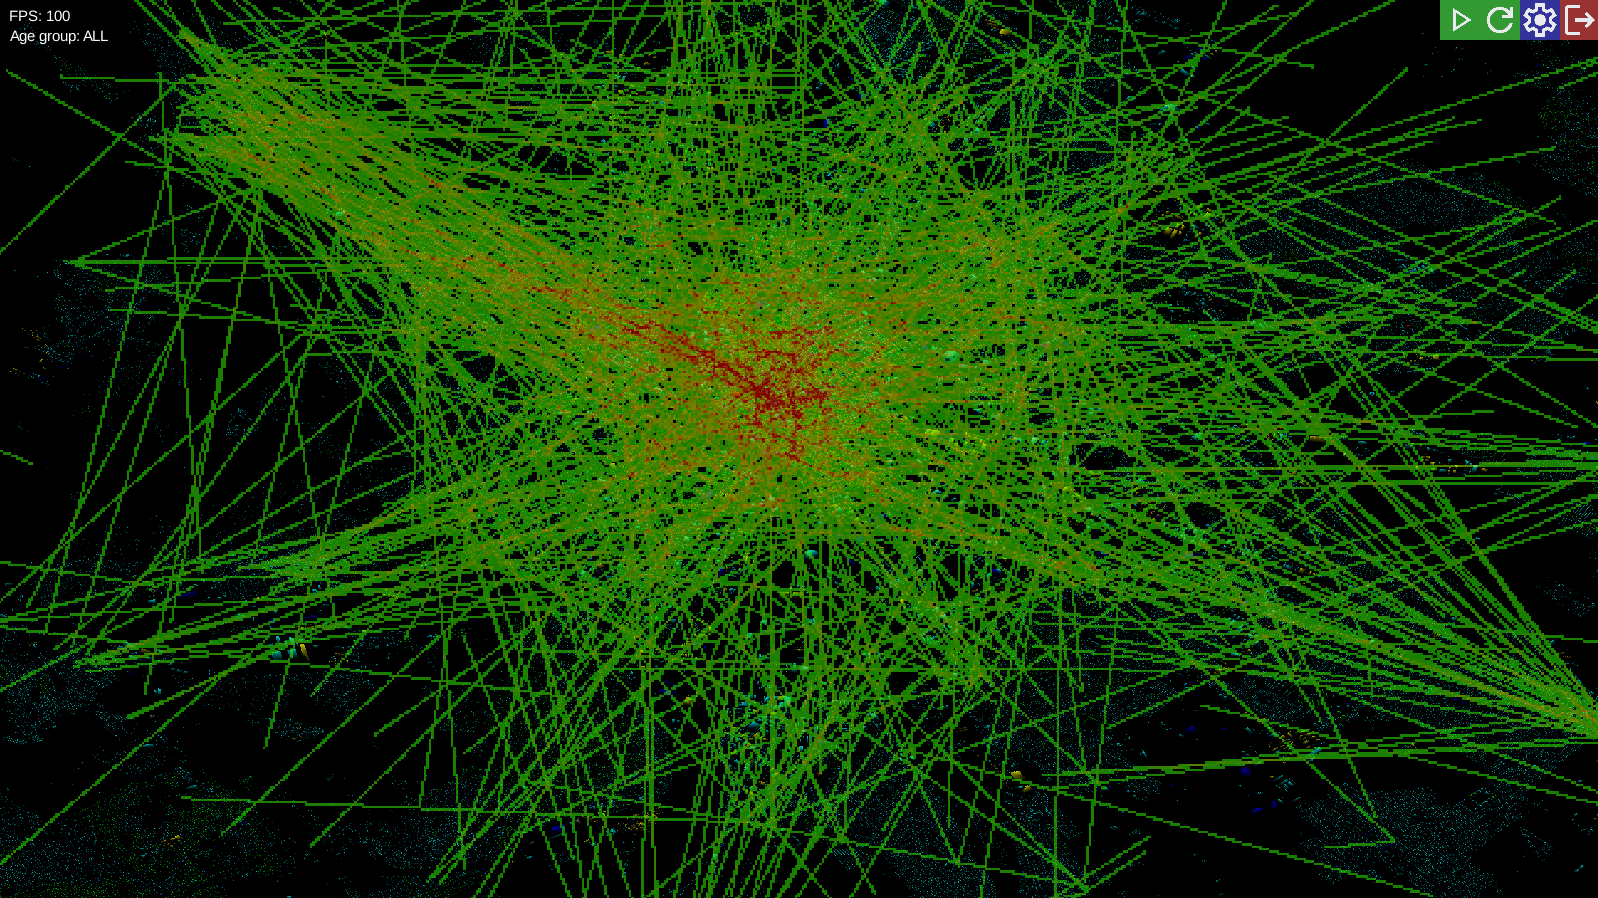
\includegraphics[width=110mm, keepaspectratio]{images/heatmap_1000.png}
    \caption{Heatmap using 1000 agents, see~\ref{perftesting-heatmap}}
\end{figure}
\begin{figure}[!h]
    \centering
    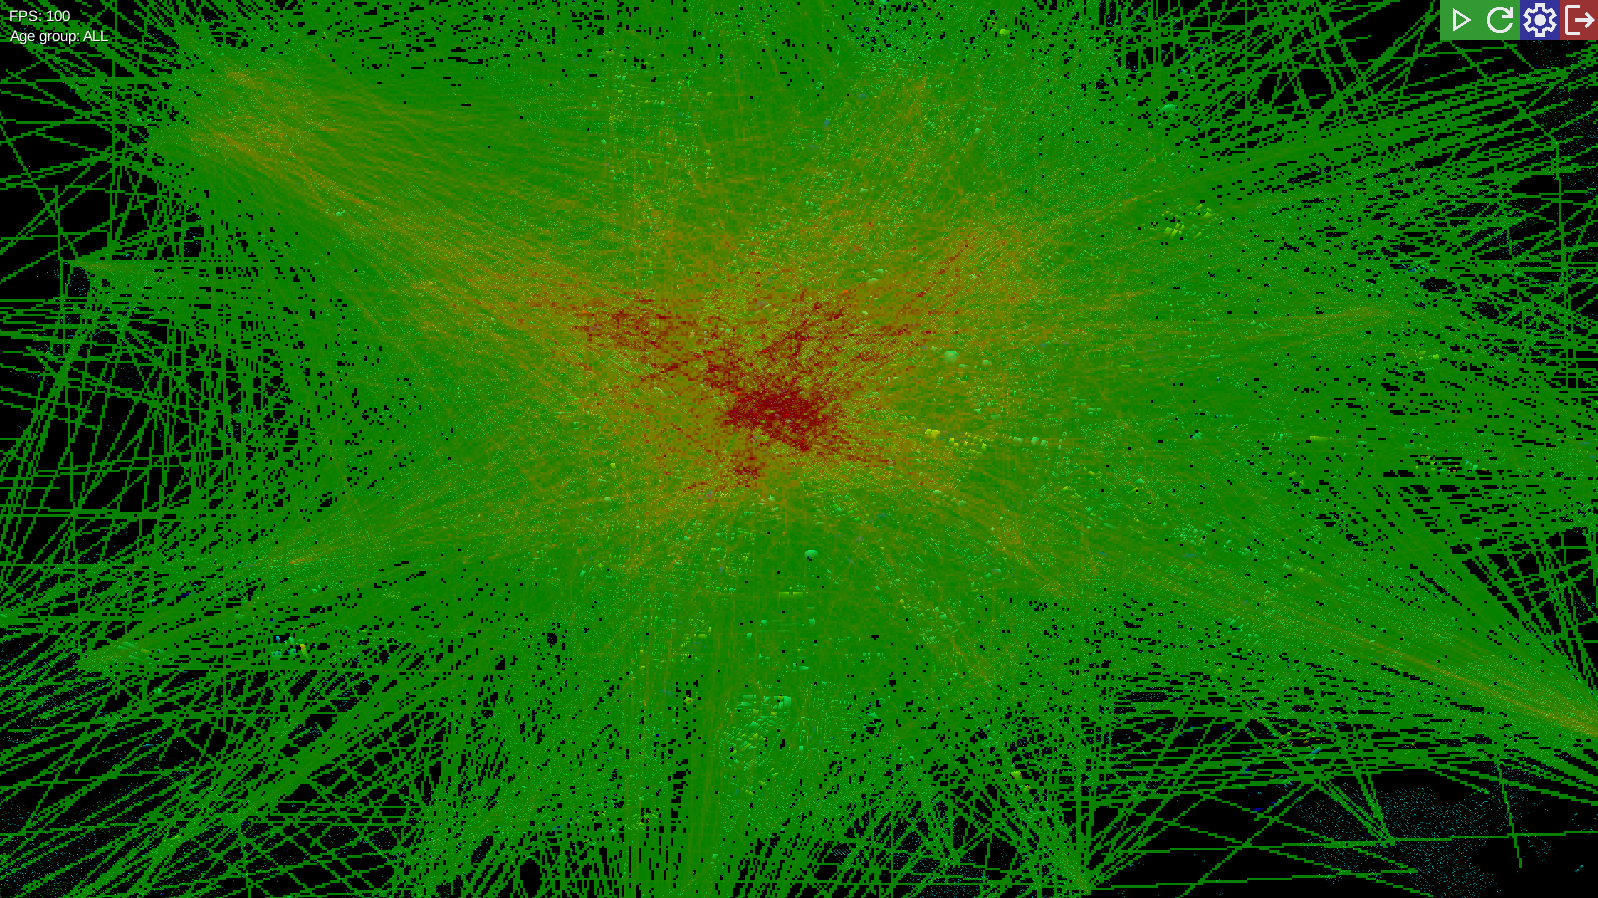
\includegraphics[width=110mm, keepaspectratio]{images/heatmap_5000.png}
    \caption{Heatmap using 5000 agents, see~\ref{perftesting-heatmap}}
\end{figure}
\begin{figure}[!h]
    \centering
    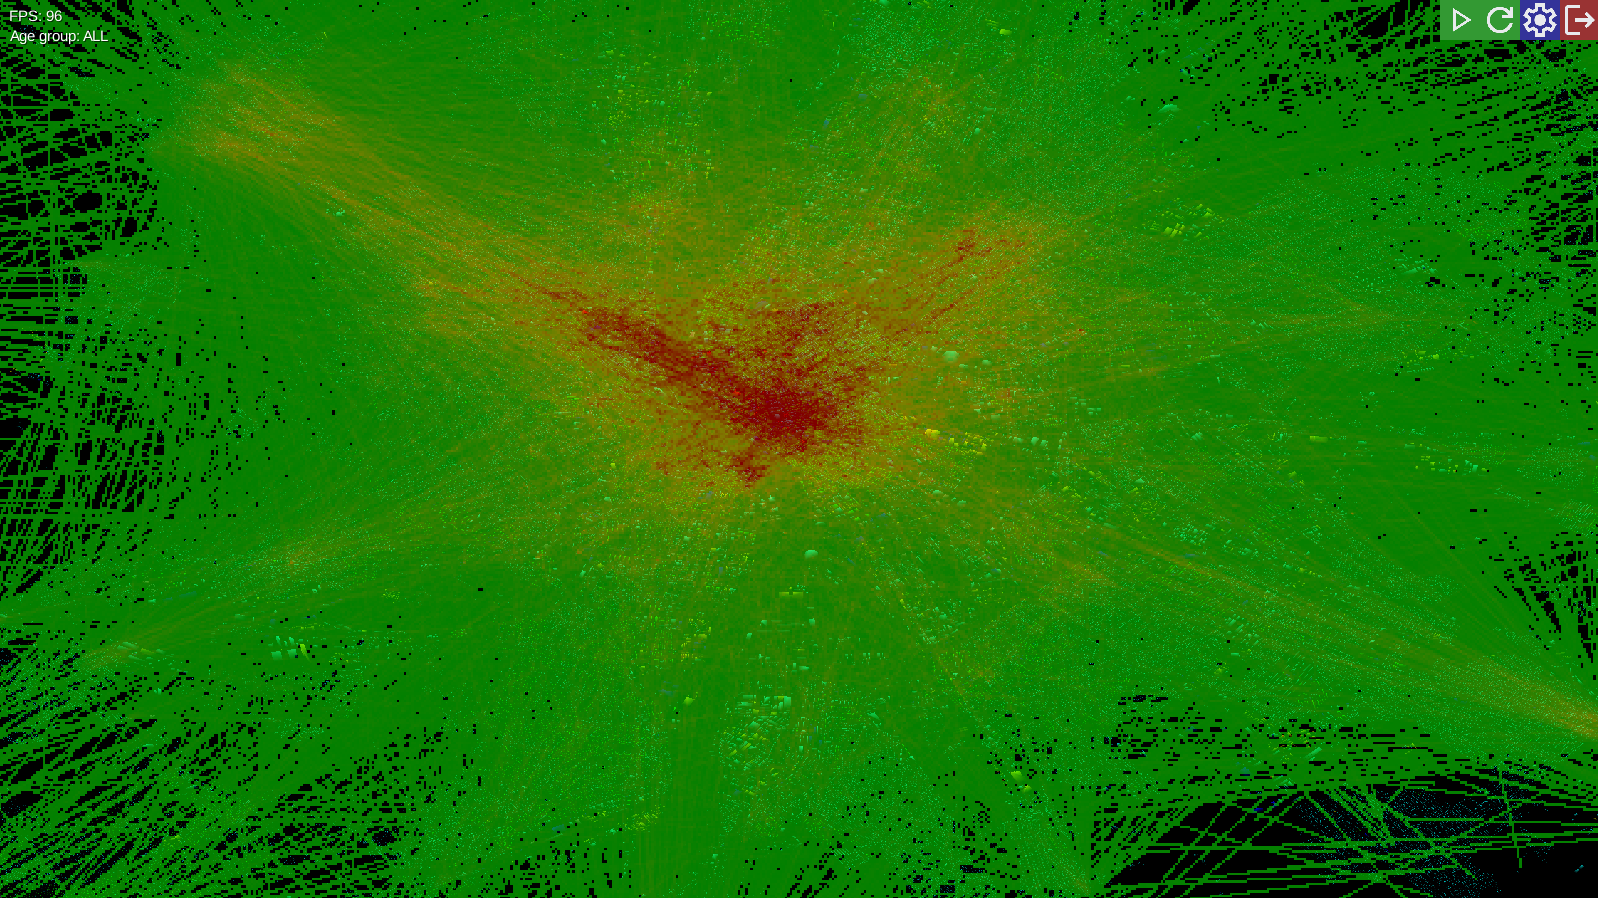
\includegraphics[width=110mm, keepaspectratio]{images/heatmap_10000.png}
    \caption{Heatmap using 10000 agents, see~\ref{perftesting-heatmap}}
\end{figure}
\begin{figure}[!h]
    \centering
    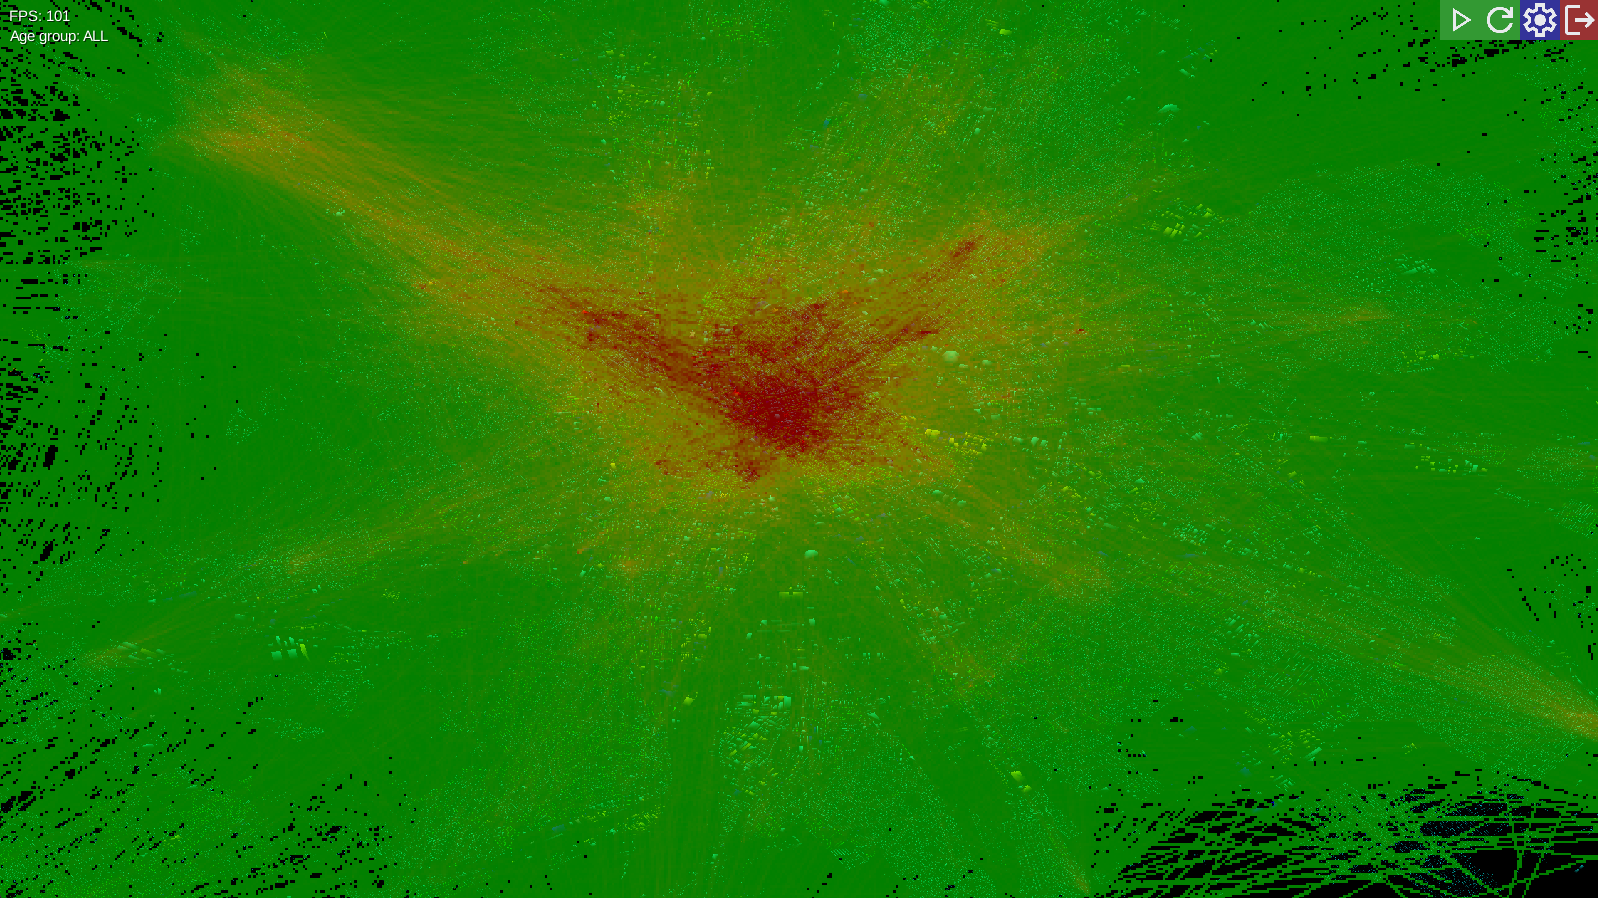
\includegraphics[width=110mm, keepaspectratio]{images/heatmap_20000.png}
    \caption{Heatmap using 20000 agents, see~\ref{perftesting-heatmap}}
\end{figure}
\begin{figure}[!h]
    \centering
    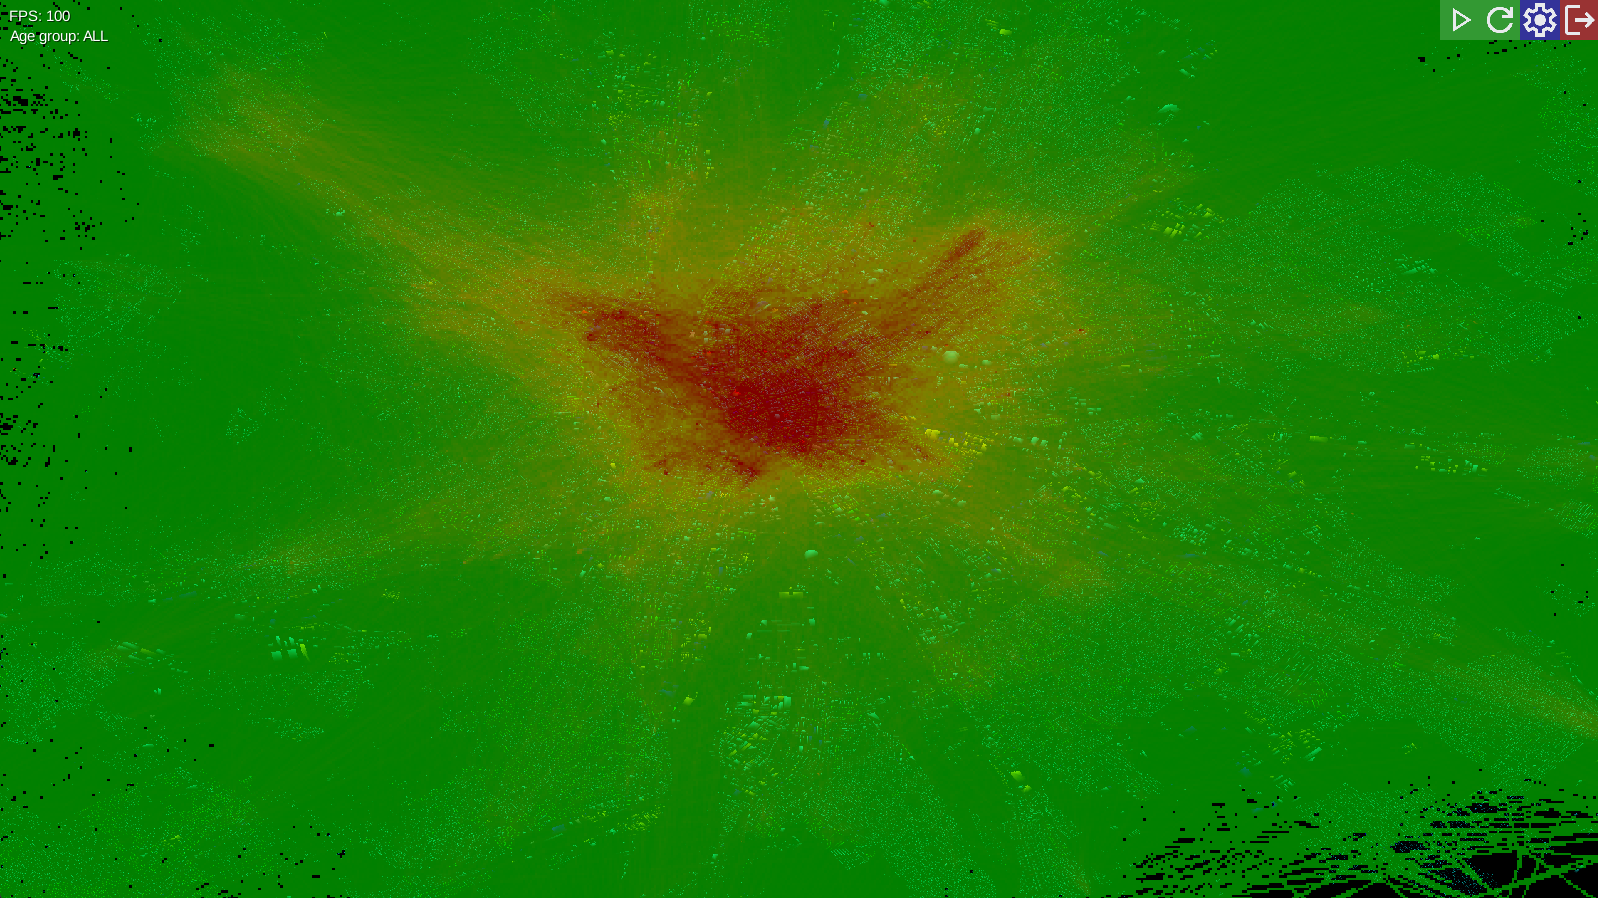
\includegraphics[width=110mm, keepaspectratio]{images/heatmap_50000.png}
    \caption{Heatmap using 50000 agents, see~\ref{perftesting-heatmap}}
\end{figure}

\label{age-groups}
\begin{figure}[!h]
    \centering
    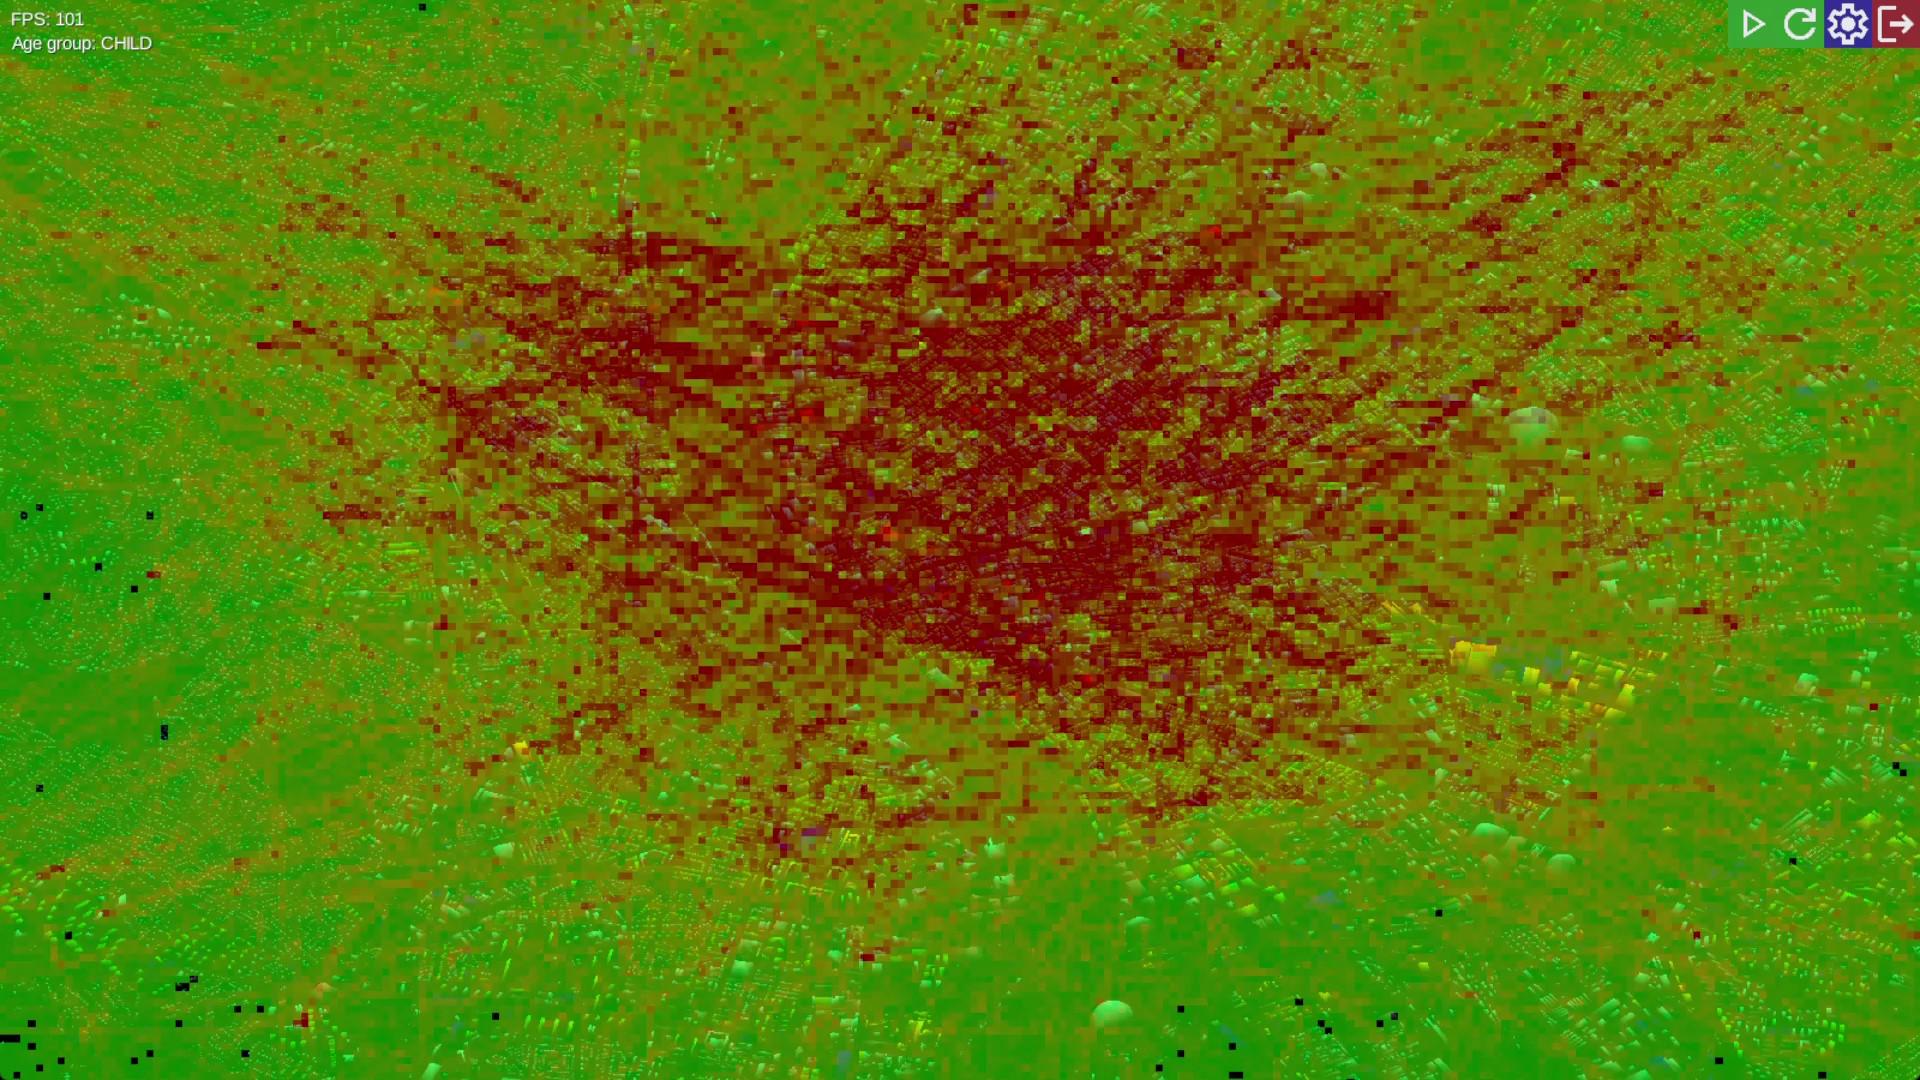
\includegraphics[width=110mm, keepaspectratio]{images/heatmap-children.jpg}
    \caption{Reference simulation heatmap, age group: children}
\end{figure}
\begin{figure}[!h]
    \centering
    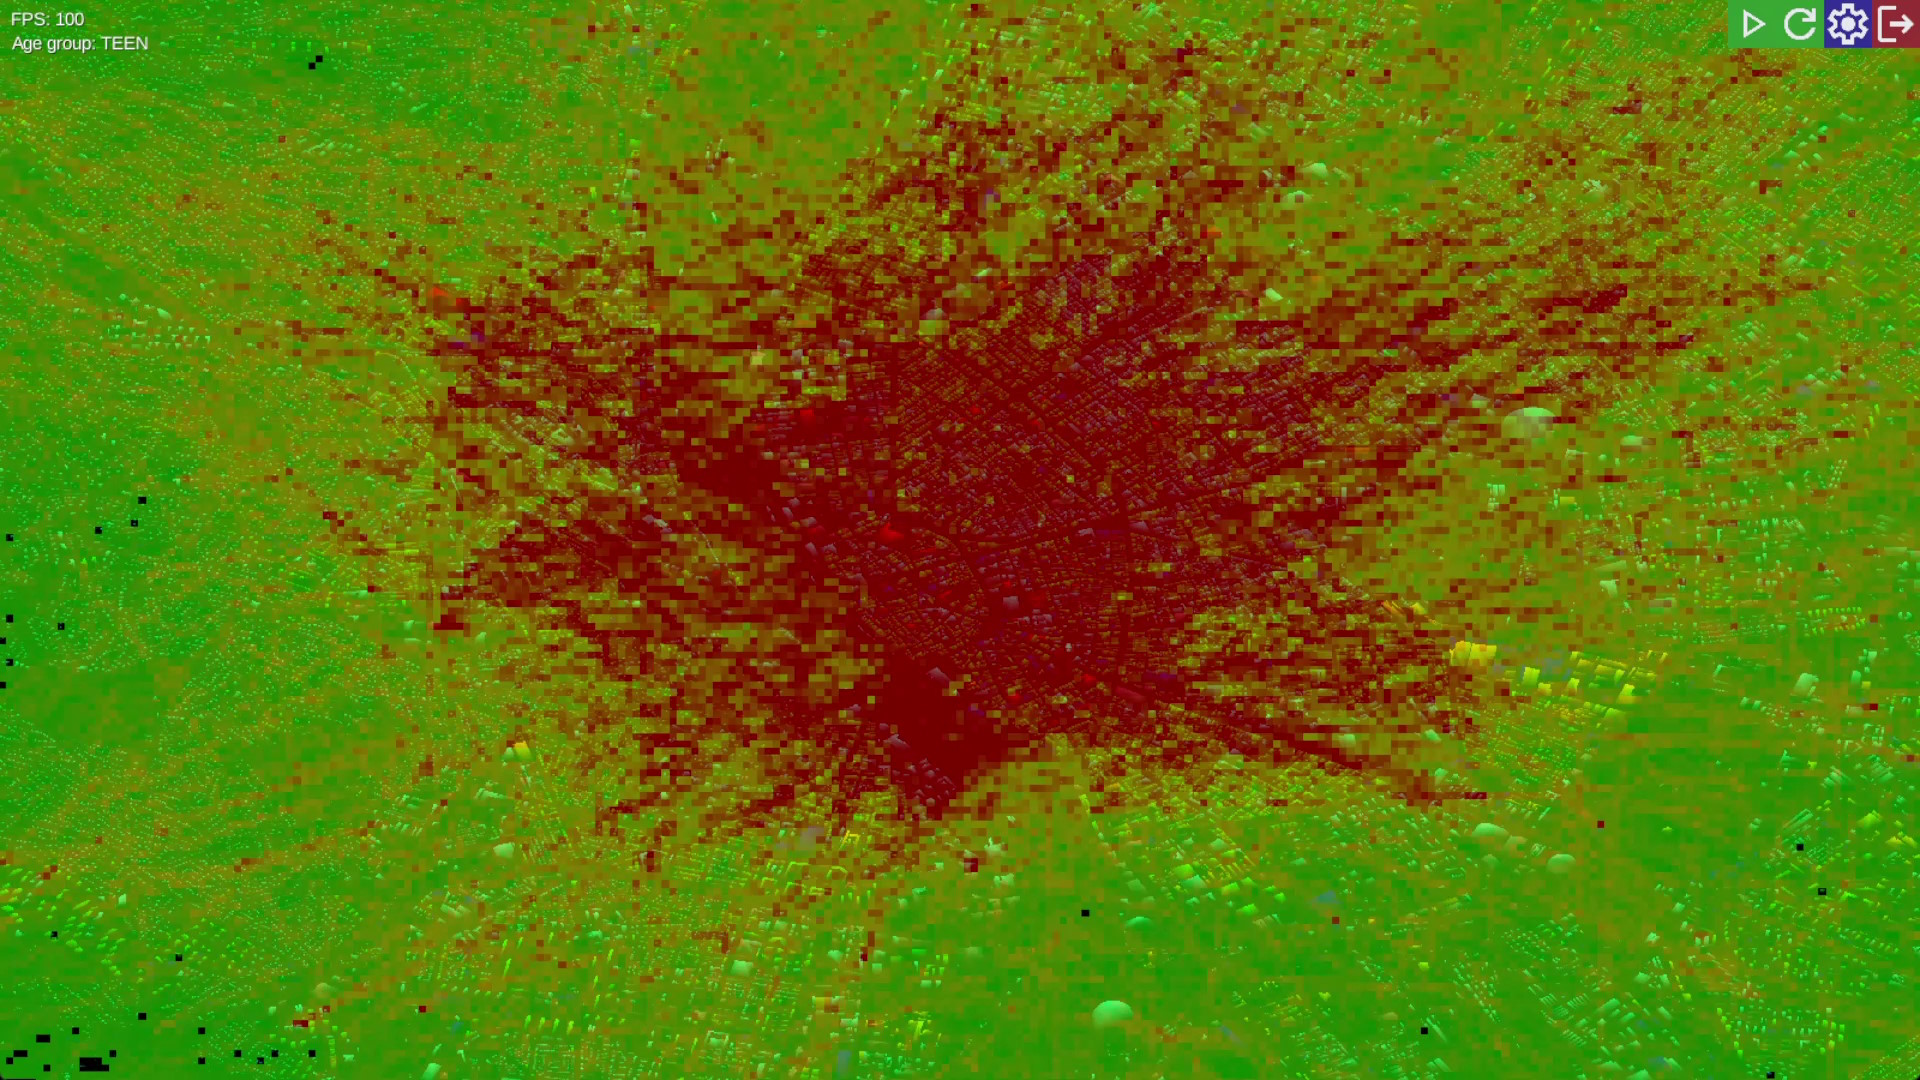
\includegraphics[width=110mm, keepaspectratio]{images/heatmap-teens.jpg}
    \caption{Reference simulation heatmap, age group: teenagers}
\end{figure}
\begin{figure}[!h]
    \centering
    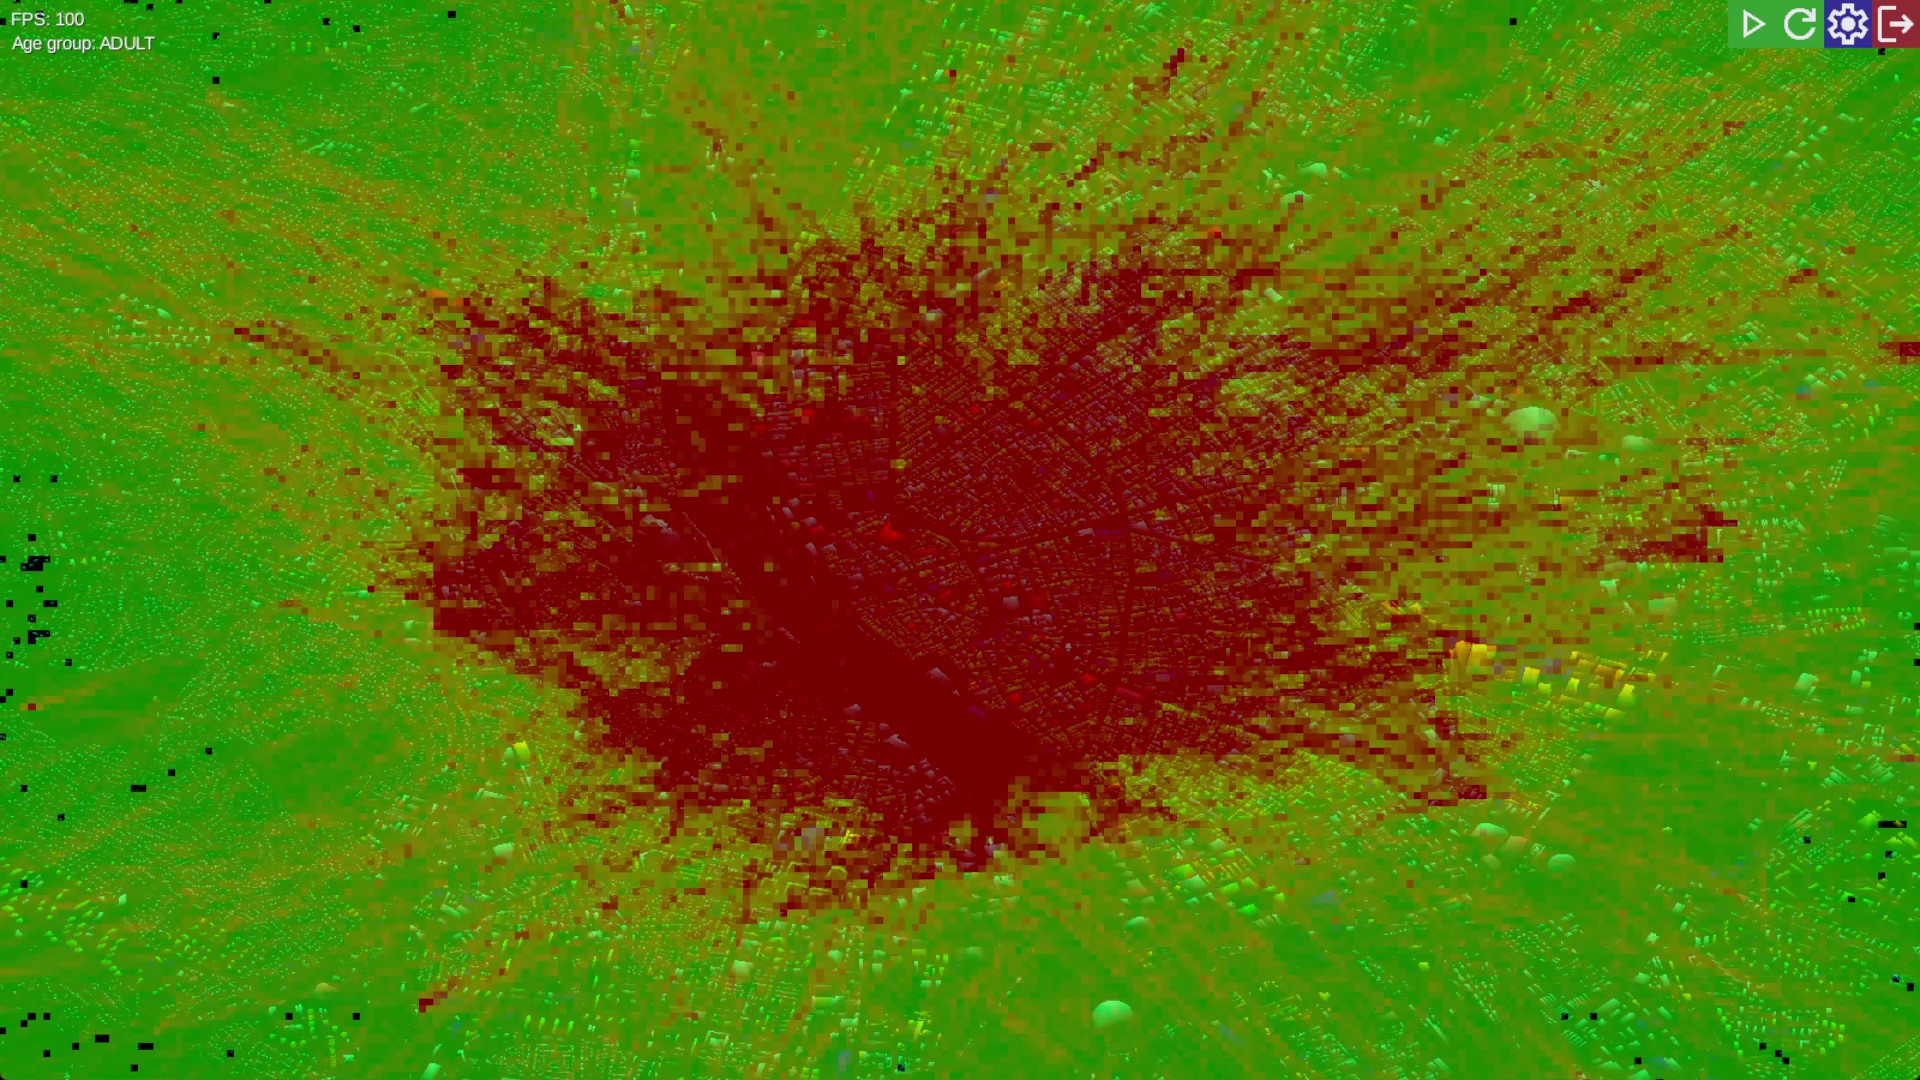
\includegraphics[width=110mm, keepaspectratio]{images/heatmap-adults.jpg}
    \caption{Reference simulation heatmap, age group: adults}
\end{figure}
\begin{figure}[!h]
    \centering
    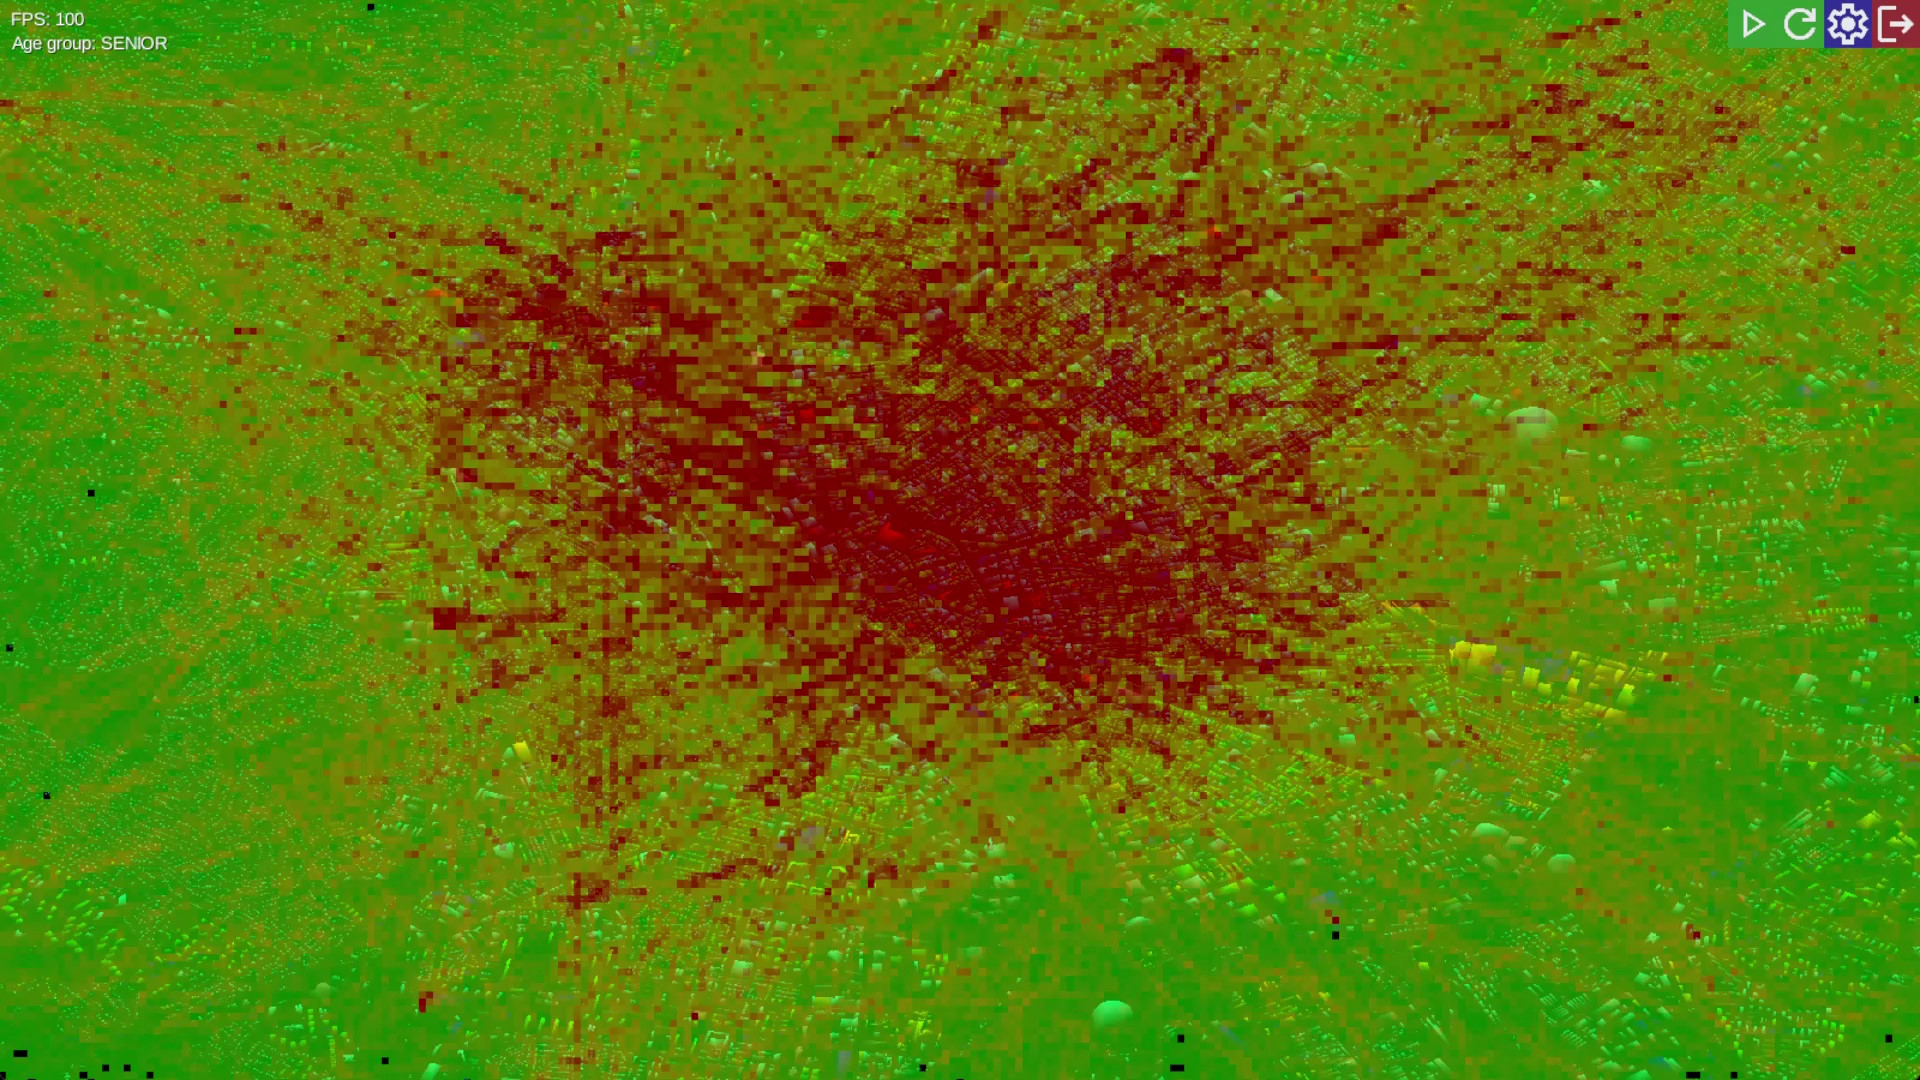
\includegraphics[width=110mm, keepaspectratio]{images/heatmap-seniors.jpg}
    \caption{Reference simulation heatmap, age group: seniors}
\end{figure}

%\label{page:last}
\end{document}
